\documentclass[11pt]{article}

\usepackage[margin=1in]{geometry}
\usepackage{amsmath,amssymb,bm}
\usepackage{graphicx}
\usepackage{booktabs}
\usepackage{array}
\usepackage{tabularx}
\usepackage{hyperref}
\usepackage{xcolor}
\usepackage{caption}
\usepackage{subcaption}
\usepackage{enumitem}

\setlist[itemize]{leftmargin=1.2em}
\setlist[enumerate]{leftmargin=1.4em}
\emergencystretch=2em

\hypersetup{
  colorlinks=true,
  linkcolor=blue!60!black,
  citecolor=blue!60!black,
  urlcolor=blue!60!black
}

\newcommand{\RR}{\mathbb{R}}
\newcommand{\bu}{\mathbf u}
\newcommand{\bc}{\mathbf c}
\newcommand{\bq}{\boldsymbol q}
\newcommand{\bz}{\boldsymbol z}
\newcommand{\bmu}{\boldsymbol\mu}
\newcommand{\boldeta}{\boldsymbol\eta}
\newcommand{\btheta}{\boldsymbol\theta}
\newcommand{\bTheta}{\boldsymbol\Theta}
\newcommand{\bQ}{\mathbf Q}
\newcommand{\bQbar}{\bar{\mathbf Q}}
\newcommand{\bdotQ}{\dot{\mathbf Q}}
\newcommand{\bone}{\mathbf 1}
\newcommand{\bzero}{\mathbf 0}
\newcommand{\bI}{\mathbf I}
\newcommand{\bV}{\mathbf V}
\newcommand{\bVbar}{\bar{\mathbf V}}
\newcommand{\Vbar}{\bVbar}
\newcommand{\bB}{\mathbf B}
\newcommand{\bA}{\mathbf A}
\newcommand{\bH}{\mathbf H}
\newcommand{\bP}{\mathbf P}
\newcommand{\bW}{\mathbf W}
\newcommand{\bXi}{\boldsymbol\Xi}
\newcommand{\bLambda}{\boldsymbol\Lambda}
\newcommand{\bPhi}{\boldsymbol\Phi}
\newcommand{\bC}{\mathbf C}
\newcommand{\bZ}{\mathbf Z}
\newcommand{\bG}{\mathbf G}
\newcommand{\bEta}{\mathbf E_\eta}
\newcommand{\bJ}{\mathbf J}
\newcommand{\qbar}{\bar{\boldsymbol q}}
\newcommand{\uref}{\mathbf u_{\mathrm{ref}}}
\newcommand{\Nmap}{\mathcal{N}}
\newcommand{\diag}{\operatorname{diag}}
\newcommand{\argmin}{\operatorname*{arg\,min}}
\newcommand{\qdim}{r}
\newcommand{\rbar}{\bar r}
\newcommand{\nmu}{n_\mu}
\newcommand{\featuredim}{F}
\newcommand{\by}{\boldsymbol y}
\newcommand{\bU}{\mathbf U}
\newcommand{\bR}{\mathbf R}

\title{\textbf{Nonlinear-Map Manifold POD Operator Inference}\\
\large A structure-preserving extension of polynomial-manifold OpInf with KdV and
parametric Burgers evidence}
\author{Draft manuscript}
\date{\today}

\begin{document}
\maketitle

\begin{abstract}
We formulate and test a nonlinear-map manifold POD operator-inference model
(NM-MPOD) for transport-dominated reduced-order modeling. The construction keeps
the modal primary/secondary split used in polynomial-manifold OpInf: the online
state is the primary coordinate vector
$\bq(t;\bmu)\in\RR^{\qdim}$, while the secondary POD coordinates are recovered
algebraically. The new ingredient is to replace the fixed polynomial secondary
map $\bXi\boldsymbol g_p(\bq)$ by a learned nonlinear map
$\Nmap(\bq,\bmu)\in\RR^{\rbar}$, represented here by Gaussian-process and
neural-network regressors.

The central algebraic point is that, for a quadratic full-order vector field, a
nonlinear split decoder changes the correct reduced operator library. Once
\[
  \bu\approx\uref+\bV\bq+\bVbar\bz,
  \qquad \bz=\Nmap(\bq,\bmu),
\]
the state-quadratic expansion contains not only $\bq\otimes\bq$ but also
$\bq\otimes\bz$ and $\bz\otimes\bz$. We therefore distinguish between
nonlinear-feature closures, which append a learned secondary feature block, and
the state-quadratically complete NM-MPOD library, which includes all three
quadratic blocks in $(\bq,\bz)$.

We use the following nomenclature throughout. The \emph{augmented-linear}
variant (AL-NM-MPOD) uses a vector field that is affine in the augmented
coordinates $[\bq^T,\bz^T]^T$. The \emph{primary-quadratic} variant
(PQ-NM-MPOD) retains the standard primary quadratic block
$\bq_{\mathrm{quad}}$ and adds $\bz$ as a nonlinear feature. The
\emph{quadratic-complete} variant (QC-NM-MPOD) is the algebraically complete
quadratic library in the augmented coordinates $[\bq^T,\bz^T]^T$.

The KdV experiments verify the nonlinear-feature and MPOD machinery on a
published soliton-style benchmark. The parametric Burgers experiments compare
three ANN-NM-MPOD dynamics libraries with $\qdim=10$ and $\rbar=133$:
QC-NM-MPOD, PQ-NM-MPOD, and AL-NM-MPOD. In the retained Burgers suite, all
three ANN-NM-MPOD variants reduce the relative rollout errors from
approximately $9\times10^{-2}$ for standard OpInf and $8\times10^{-2}$ for
polynomial MPOD to the $10^{-2}$--$10^{-3}$ range. The QC variant has the best
average error, about $6\times10^{-3}$, but it uses a much larger operator
library: $10495$ inferred right-hand-side features versus $199$ for AL-NM-MPOD,
$254$ for PQ-NM-MPOD, $121$ for standard quadratic OpInf, and $276$ for MPOD
with $p=2$.
\end{abstract}

\section{Overview and contributions}

The proposed reduced representation is
\begin{equation}
  \bu(t;\bmu) \approx \uref + \bV\bq(t;\bmu) + \bVbar \Nmap(\bq(t;\bmu),\bmu),
  \label{eq:nmmpod_decoder}
\end{equation}
with $\bV\in\RR^{N\times \qdim}$, $\bVbar\in\RR^{N\times \rbar}$, and
\begin{equation}
  \Nmap:\RR^{\qdim+\nmu}\rightarrow \RR^{\rbar}.
\end{equation}
Only $\bq(t;\bmu)\in\RR^{\qdim}$ is evolved by the online ODE. The vector
$\qbar(t;\bmu)=\Nmap(\bq(t;\bmu),\bmu)$ supplies the coefficients of the
secondary POD modes. In the retained Burgers experiments,
\[
  \qdim=10,\qquad \rbar=133,\qquad \qdim+\rbar=143.
\]

The three central claims are:
\begin{enumerate}
  \item The idea is a direct generalization of the MPOD decoder: replace the
  polynomial secondary-coordinate map $\bXi \boldsymbol g(\bq)$ by a learned
  nonlinear map $\Nmap(\bq,\bmu)$ while retaining a modal primary/secondary
  decomposition.
  \item For a quadratic full-order vector field and the modal projection used
  here, the state-quadratically complete library is not just
  $\bq\otimes\bq$. It also includes
  $\bq\otimes \Nmap(\bq,\bmu)$ and
  $\Nmap(\bq,\bmu)\otimes \Nmap(\bq,\bmu)$.
  \item The full NM-MPOD library is faithful to the quadratic algebra, but much
  larger than the standard linear-subspace library. In the Burgers case the
  feature count is 10495 for QC-NM-MPOD versus 254 for PQ-NM-MPOD, 199 for
  AL-NM-MPOD, 121 for standard quadratic OpInf, and 276 for induced MPOD with
  $p=2$. This makes regularization and validation central rather than optional.
\end{enumerate}

\begin{table}[ht]
\centering
\caption{Notation used throughout the manuscript. Vectors and matrices are bold;
plain symbols denote scalar dimensions or scalar hyperparameters.}
\label{tab:notation}
\begin{tabularx}{\textwidth}{p{0.20\textwidth}X}
\toprule
Symbol & Meaning\\
\midrule
$\bu(t;\bmu)\in\RR^N$ & Semidiscrete full-order state.\\
$\bmu\in\RR^{\nmu}$ & Physical parameter vector; for Burgers,
$\bmu=(\mu_1,\mu_2)^T$.\\
$\boldeta(\bmu)\in\RR^m$ & Chosen parameter feature vector; in Burgers
$m=5$ and $\boldeta=[\mu_1,\mu_2,\mu_1^2,\mu_1\mu_2,\mu_2^2]^T$.\\
$\bV\in\RR^{N\times\qdim}$ & Primary POD basis; $\bq(t;\bmu)$ are the evolved
coordinates.\\
$\bVbar\in\RR^{N\times\rbar}$ & Secondary POD basis; $\qbar(t;\bmu)$ is
reconstructed algebraically.\\
$\boldsymbol g_p(\bq)$ & Polynomial MPOD decoder features.\\
$\hat{\boldsymbol g}(\bq)$ & Higher monomials induced in the reduced vector
field after substituting the MPOD decoder into a quadratic FOM.\\
$\Nmap(\bq,\bmu)$ & Learned secondary-coordinate map for NM-MPOD.\\
$\btheta(\bq,\bmu)$ & OpInf right-hand-side feature vector.\\
$\bW$ & Inferred reduced operator matrix satisfying
$\dot{\bq}\approx\bW\btheta(\bq,\bmu)$.\\
\bottomrule
\end{tabularx}
\end{table}

\section{Relationship to nonlinear-manifold OpInf}

Geelen, Balzano, Wright, and Willcox formulate nonlinear modal state
approximations of the form
\begin{equation}
  \mathbf s(t) \approx \mathbf s_{\mathrm{ref}}
  + \bV\hat{\mathbf s}(t)
  + \bVbar \bXi \boldsymbol g(\hat{\mathbf s}(t)),
  \label{eq:paper_decoder}
\end{equation}
where $\bV$ contains primary modal directions, $\bVbar$ contains additional
orthogonal directions, and $\boldsymbol g$ is typically a low-order polynomial
embedding \cite{geelen2024learning}. The present study uses the POD-based construction:
$\bV$ and $\bVbar$ are selected from the POD hierarchy. The corresponding
polynomial-manifold baseline is MPOD-OpInf.

The proposed NM-MPOD approximation keeps the modal structure in
\eqref{eq:paper_decoder}, but replaces the fixed polynomial map:
\begin{equation}
  \bXi \boldsymbol g(\bq) \quad \leadsto \quad \Nmap(\bq,\bmu).
\end{equation}
Thus, the decoder becomes \eqref{eq:nmmpod_decoder}. This differs from a generic
autoencoder ROM in three important ways:
\begin{enumerate}
  \item The basis matrices $\bV$ and $\Vbar$ remain modal and interpretable.
  \item The online state dimension is still $r$, not $r+\bar r$.
  \item The reduced dynamics can still be learned with an OpInf library whose
  algebraic terms are chosen from the structure of the governing equations.
\end{enumerate}

\section{Benchmark problems and semidiscrete structure}

Both benchmarks considered here lead to reduced vector-field libraries governed
by quadratic nonlinearities. This is the key structural fact behind the
operator choices in the remainder of the study.

\subsection{Periodic KdV soliton}

The first benchmark is the periodic Korteweg--de Vries equation
\begin{equation}
  s_t + \alpha s s_x + \beta s_{xxx}=0,
  \qquad x\in[-\pi,\pi),\qquad t\in[0,1],
  \label{eq:kdv_pde}
\end{equation}
with periodic boundary conditions, $\alpha=4$, $\beta=1$, and initial condition
\begin{equation}
  s(x,0)=1+24\,\mathrm{sech}^2(\sqrt{8}\,x).
  \label{eq:kdv_ic}
\end{equation}
The full-order data are generated with a Fourier pseudospectral spatial
discretization using $N=256$ grid points and an exponential time-differencing
Runge--Kutta method with time step $\Delta t=2\times10^{-4}$. The interval
$t\in[0,0.2]$ is used for training and $t\in(0.2,1]$ is treated as prediction.
After spatial discretization, the nonlinear term $s s_x$ is quadratic in the
state, so the semidiscrete dynamics have the schematic form
\begin{equation}
  \dot{\bu}=\bA\bu+\bH(\bu\otimes\bu).
  \label{eq:kdv_semidiscrete}
\end{equation}

\subsection{Parametric inviscid Burgers equation}

The second benchmark is a parametric one-dimensional inviscid Burgers problem
on $x\in[0,100]$,
\begin{equation}
  u_t + \left(\frac{u^2}{2}\right)_x = 0.02\,\exp(\mu_2 x),
  \qquad
  u(x,0)=1,
  \label{eq:burgers_pde}
\end{equation}
with a left inflow state controlled by $\mu_1$, equivalently a left boundary
flux $f(u(0,t))=\mu_1^2/2$. The parameter vector is
\begin{equation}
  \bmu=(\mu_1,\mu_2)^T,\qquad
  \mu_1\in[4.25,5.50],\qquad
  \mu_2\in[0.015,0.030].
\end{equation}
The full-order model is a first-order finite-volume discretization with
$N=5000$ cells and backward Euler time integration with $\Delta t=0.05$ over
500 time steps. For a cell-centered state $\bu^n$, one backward Euler step
solves a nonlinear residual of the form
\begin{equation}
  R_i(\bu^{n+1};\bu^n,\bmu)
  =
  u_i^{n+1}-u_i^n
  +
  \frac{\Delta t}{\Delta x_i}
  \left(
  f(u_i^{n+1})-f(u_{i-1}^{n+1})
  \right)
  -
  \Delta t\,0.02\,\exp(\mu_2 x_i)
  =0,
  \label{eq:burgers_residual}
\end{equation}
with $f(u)=u^2/2$ and $f(u_0^{n+1})=\mu_1^2/2$ at the inflow boundary. The
nonlinear flux is quadratic in the state and the source/boundary terms encode
the parameter dependence. The nonintrusive OpInf models represent parameter
dependence through
\begin{equation}
  \boldeta(\bmu) =
  \begin{bmatrix}
  \mu_1 & \mu_2 & \mu_1^2 & \mu_1\mu_2 & \mu_2^2
  \end{bmatrix}^T.
  \label{eq:param_features}
\end{equation}

\subsection{Quadratic semidiscrete template}

Suppressing parameter dependence, both examples may be interpreted through the
quadratic semidiscrete template
\begin{equation}
  \dot{\bu} = \bc + \bA\bu + \bH(\bu\otimes \bu),
  \label{eq:fom_quadratic}
\end{equation}
with $\bu(t)\in\RR^N$. The OpInf models are nonintrusive: the matrices
$\bc$, $\bA$, and $\bH$ are not assembled. Their algebraic structure is used
only to choose reduced regression libraries. For example, the standard
linear-subspace Burgers baseline uses
\begin{equation}
  \bu \approx \uref + \bV\bq,\qquad
  \dot{\bq} = \bW\btheta(\bq,\bmu),
\end{equation}
with
\begin{equation}
  \btheta(\bq,\bmu)=
  \begin{bmatrix}
  1\\
  \boldeta(\bmu)\\
  \bq\\
  \boldeta(\bmu)\otimes \bq\\
  \bq_{\mathrm{quad}}
  \end{bmatrix}.
  \label{eq:standard_opinf}
\end{equation}
Here $\bq_{\mathrm{quad}}$ denotes the vector of unique products $q_iq_j$ for
$i\leq j$.

\section{Projected algebra: linear POD, MPOD, and NM-MPOD}
\label{sec:projected_algebra}

This section spells out the algebra that motivates the operator libraries. The
formulas are written as if the semidiscrete operators $\bc,\bA,\bH$ were known, but
the actual computation remains nonintrusive: OpInf only uses the resulting term
structure to choose a regression library.

For readability, parameter dependence is suppressed in the derivation. The
analysis therefore begins from
\begin{equation}
  \dot{\bu} = \bc + \bA\bu + \bH(\bu\otimes \bu),
  \label{eq:quadratic_fom_no_mu}
\end{equation}
with $\bu(t)\in\RR^N$, $\bA\in\RR^{N\times N}$, and
$\bH\in\RR^{N\times N^2}$. Parameter features such as $\boldeta(\bmu)$ are then added
to the inferred library for the parametric Burgers problem.

\subsection{Standard linear-subspace OpInf}

For the standard POD approximation,
\begin{equation}
  \bu(t) \approx \uref + \bV\bq(t),
  \qquad
  \bV\in\RR^{N\times \qdim},
  \qquad
  \bV^T\bV=\bI.
  \label{eq:linear_decoder_derivation}
\end{equation}
The time derivative is
\begin{equation}
  \dot{\bu} = \bV\dot{\bq}.
\end{equation}
Projecting \eqref{eq:quadratic_fom_no_mu} with $\bV^T$ gives
\begin{equation}
  \dot{\bq}
  =
  \bV^T \bc
  + \bV^T \bA(\uref+\bV\bq)
  + \bV^T \bH\left((\uref+\bV\bq)\otimes(\uref+\bV\bq)\right).
\end{equation}
Now expand the Kronecker product:
\begin{align}
  (\uref+\bV\bq)\otimes(\uref+\bV\bq)
  ={}&
  \uref\otimes\uref
  + \uref\otimes \bV\bq
  + \bV\bq\otimes \uref
  + \bV\bq\otimes \bV\bq.
\end{align}
Therefore the reduced equation can be grouped as
\begin{equation}
  \dot{\bq} = \hat{\bc} + \hat{\bA}\bq + \hat{\bH}(\bq\otimes\bq),
  \label{eq:linear_pod_grouped}
\end{equation}
where the intrusive expressions would be
\begin{align}
  \hat{\bc}
  &=
  \bV^T\left(\bc + \bA\uref + \bH(\uref\otimes\uref)\right),\\
  \hat{\bA}\bq
  &=
  \bV^T \bA \bV\bq
  + \bV^T \bH(\uref\otimes \bV\bq)
  + \bV^T \bH(\bV\bq\otimes \uref),\\
  \hat{\bH}(\bq\otimes\bq)
  &=
  \bV^T \bH(\bV\bq\otimes \bV\bq).
\end{align}
The important consequence is simple: a quadratic FOM and a linear decoder
produce only constant, linear, and quadratic functions of the primary
coordinates $\bq$. This is the reason the standard OpInf model uses the library
\[
  \btheta_{\mathrm{lin}}(\bq,\bmu)=
  \begin{bmatrix}
  1 & \boldeta(\bmu) & \bq & \boldeta(\bmu)\otimes\bq & \bq_{\mathrm{quad}}
  \end{bmatrix}^T.
\]

\subsection{Polynomial MPOD-OpInf}

The MPOD nonlinear manifold used in nonlinear-manifold OpInf has the form
\begin{equation}
  \bu(t) \approx \uref + \bV\bq(t) + \Vbar \bz_p(\bq(t)),
  \qquad
  \bz_p(\bq)=\bXi \boldsymbol g_p(\bq),
  \label{eq:mpod_decoder_derivation}
\end{equation}
where $\bV\in\RR^{N\times \qdim}$ contains primary POD modes,
$\Vbar\in\RR^{N\times \rbar}$ contains secondary POD modes, and
$\bV^T\Vbar=\bzero$. The vector $\boldsymbol g_p(\bq)$ contains polynomial
features up to degree $p$, usually starting at degree two. Thus $\bz_p(\bq)$ is
not evolved by an ODE; it is reconstructed algebraically from $\bq$.

The left-hand side is where an important Willcox-style simplification enters.
By the chain rule,
\begin{equation}
  \dot{\bu}
  =
  \bV\dot{\bq} + \bVbar \frac{\partial \bz_p}{\partial \bq}(\bq)\dot{\bq}.
\end{equation}
Projecting with $\bV^T$ gives
\begin{equation}
  \bV^T\dot{\bu}
  =
  \bV^T\bV\dot{\bq}
  +
  \bV^T\bVbar \frac{\partial \bz_p}{\partial \bq}(\bq)\dot{\bq}
  =
  \dot{\bq}.
  \label{eq:modal_projection_cancels_tangent}
\end{equation}
So under modal projection with orthogonal $\bV$ and $\Vbar$, the nonlinear
tangent term does not appear on the left-hand side. If instead one used a
tangent-space projection, a state-dependent mass matrix would appear. The
present study follows the modal projection structure used in the
nonlinear-manifold OpInf construction.

Now define the combined modal coordinate
\begin{equation}
  \boldsymbol y(\bq)=
  \begin{bmatrix}
  \bq\\ \bz_p(\bq)
  \end{bmatrix},
  \qquad
  \bB =
  \begin{bmatrix}
  \bV & \Vbar
  \end{bmatrix},
  \qquad
  \bu=\uref+\bB\boldsymbol y.
\end{equation}
Substituting into the projected FOM gives
\begin{equation}
  \dot{\bq}
  =
  \bV^T \bc
  + \bV^T \bA(\uref+\bV\boldsymbol y_q+\Vbar\boldsymbol y_z)
  + \bV^T \bH\left((\uref+\bV\boldsymbol y_q+\Vbar\boldsymbol y_z)
  \otimes
  (\uref+\bV\boldsymbol y_q+\Vbar\boldsymbol y_z)\right),
  \label{eq:mpod_substituted}
\end{equation}
where $\boldsymbol y_q=\bq$ and $\boldsymbol y_z=\bz_p(\bq)$. Expanding the
quadratic term gives
\begin{align}
  \bu\otimes\bu
  ={}&
  \uref\otimes\uref
  + \uref\otimes \bV\bq
  + \bV\bq\otimes\uref
  + \uref\otimes \Vbar\bz_p
  + \Vbar\bz_p\otimes\uref
  \notag\\
  &+
  \bV\bq\otimes \bV\bq
  + \bV\bq\otimes \Vbar\bz_p
  + \Vbar\bz_p\otimes \bV\bq
  + \Vbar\bz_p\otimes \Vbar\bz_p.
  \label{eq:mpod_full_kron_expansion}
\end{align}
After applying $\bV^T\bA$ and $\bV^T\bH$, the projected dynamics have the split form
\begin{align}
  \dot{\bq}
  ={}&
  \bc_0
  + \bA_q \bq
  + \bA_z \bz_p(\bq)
  + \bH_{qq}(\bq\otimes\bq)
  \notag\\
  &+
  \bH_{qz}\bigl(\bq\otimes\bz_p(\bq)\bigr)
  + \bH_{zz}\bigl(\bz_p(\bq)\otimes\bz_p(\bq)\bigr).
  \label{eq:mpod_split_form}
\end{align}
Here $\bH_{qz}$ absorbs both cross terms
$\bV\bq\otimes \Vbar\bz_p$ and $\Vbar\bz_p\otimes \bV\bq$; formally this uses a
permutation between $\bz_p\otimes\bq$ and $\bq\otimes\bz_p$.

Equation \eqref{eq:mpod_split_form} is the expanded version. The Willcox
polynomial-manifold model often writes the same content after regrouping by
polynomial degree:
\begin{equation}
  \dot{\bq}
  =
  \hat{\bc}
  + \hat{\bA}\bq
  + \hat{\bH}(\bq\otimes\bq)
  + \hat{\bP}\,\hat{\boldsymbol g}(\bq).
  \label{eq:willcox_grouped_polynomial}
\end{equation}
The subtle point is that $\hat{\boldsymbol g}(\bq)$ is not necessarily the same
vector as the decoder feature vector $\boldsymbol g_p(\bq)$. It collects the higher-order monomials induced
by the substituted nonlinear manifold and by the quadratic FOM. For example, if
$\bz_p(\bq)$ contains polynomial terms of degrees $2,\ldots,p$, then:
\begin{itemize}
  \item $\bA_z\bz_p(\bq)$ contributes degrees $2,\ldots,p$;
  \item $\bq\otimes\bz_p(\bq)$ contributes degrees $3,\ldots,p+1$;
  \item $\bz_p(\bq)\otimes\bz_p(\bq)$ contributes degrees $4,\ldots,2p$.
\end{itemize}
The degree-two parts can be absorbed into $\hat{\bH}(\bq\otimes\bq)$, while the
remaining degree-three through degree-$2p$ terms are collected in
$\hat{\bP}\,\hat{\boldsymbol g}(\bq)$. This is the origin of the higher-order polynomial operator
in MPOD-OpInf.

\subsection{Nonlinear-map MPOD}

The proposed NM-MPOD decoder keeps the same modal split but replaces the fixed
polynomial map by a learned map:
\begin{equation}
  \bu(t;\bmu)
  \approx
  \uref + \bV\bq(t;\bmu) + \Vbar\bz(t;\bmu),
  \qquad
  \bz(t;\bmu)=\Nmap(\bq(t;\bmu),\bmu).
  \label{eq:nmmpod_decoder_derivation}
\end{equation}
The chain-rule calculation is identical:
\begin{equation}
  \dot{\bu}
  =
  \bV\dot{\bq}
  +
  \Vbar
  \frac{\partial \Nmap}{\partial \bq}(\bq,\bmu)\dot{\bq},
\end{equation}
and modal projection again gives
\begin{equation}
  \bV^T\dot{\bu}=\dot{\bq}
  \qquad
  \text{if } \bV^T\Vbar=\bzero.
\end{equation}
Thus the Jacobian of the learned secondary map is not needed in this
modal-projection
OpInf construction.

Substitution into the quadratic FOM gives exactly the same split algebra as
\eqref{eq:mpod_split_form}, but now $\bz=\Nmap(\bq,\bmu)$ is not a known polynomial:
\begin{align}
  \dot{\bq}
  ={}&
  \bc_0
  + \bA_q \bq
  + \bA_z \bz
  + \bH_{qq}(\bq\otimes\bq)
  \notag\\
  &+
  \bH_{qz}(\bq\otimes\bz)
  + \bH_{zz}(\bz\otimes\bz),
  \qquad \bz=\Nmap(\bq,\bmu).
  \label{eq:nmmpod_full_split_form}
\end{align}
Equivalently, the quadratic expansion before grouping is
\begin{align}
  \bu\otimes\bu
  ={}&
  \uref\otimes\uref
  + \uref\otimes \bV\bq
  + \bV\bq\otimes\uref
  + \uref\otimes \Vbar\bz
  + \Vbar\bz\otimes\uref
  \notag\\
  &+
  \bV\bq\otimes \bV\bq
  + \bV\bq\otimes \Vbar\bz
  + \Vbar\bz\otimes \bV\bq
  + \Vbar\bz\otimes \Vbar\bz.
  \label{eq:full_expansion}
\end{align}
This is why adding only $\bq\otimes\bq$ is not the complete quadratic expansion
once the decoder contains a secondary nonlinear map.

Because $\bz=\Nmap(\bq,\bmu)$ is arbitrary,
\eqref{eq:nmmpod_full_split_form} cannot be reduced to a finite polynomial in
$\bq$ of known degree.
The final NM-MPOD model therefore uses an OpInf feature library built from the
observable reduced quantities $\bq$, $\bmu$, and
$\bz=\Nmap(\bq,\bmu)$:
\begin{equation}
  \btheta_{\mathrm{NM}}
  =
  \begin{bmatrix}
  1\\
  \boldeta(\bmu)\\
  \bq\\
  \boldeta(\bmu)\otimes \bq\\
  \bq_{\mathrm{quad}}\\
  \bz\\
  \bq\otimes \bz\\
  \bz_{\mathrm{quad}}
  \end{bmatrix}.
  \label{eq:full}
\end{equation}
Here $\bq_{\mathrm{quad}}$ and $\bz_{\mathrm{quad}}$ denote vectors of unique
products $q_iq_j$ and $z_iz_j$ for $i\leq j$. The library \eqref{eq:full} is
the state-quadratic completion of the quadratic FOM after the split decoder
\eqref{eq:nmmpod_decoder_derivation}.

\subsection{Why not always use the full library?}

The QC library \eqref{eq:full} is the most faithful state-quadratic expansion
of \eqref{eq:full_expansion}. However, it is also much larger. If
$\qdim=10$ and $\rbar=133$, then
\[
  \dim(\bq_{\mathrm{quad}})=\frac{10\cdot11}{2}=55,
\]
\[
  \dim(\bq\otimes\bz)=10\cdot133=1330,
\]
\[
  \dim(\bz_{\mathrm{quad}})=\frac{133\cdot134}{2}=8911.
\]
The QC ANN-NM-MPOD Burgers library therefore has 10495 scalar features.
Because only 4509 time samples are available in the nine training trajectories,
the regression is underdetermined unless strongly regularized. The
quadratic-complete Burgers fit is therefore solved in an equivalent dual ridge
form.

There are also two scope boundaries. First, \eqref{eq:full} is a
state-quadratic completion, not a complete parametric-operator expansion. A
fully expanded parametric quadratic model would also consider parameter
interactions with $\bz$, $\bq\otimes\bz$, and $\bz\otimes\bz$, depending on how
parameter dependence enters the semidiscrete operators. These terms are excluded
from the present Burgers experiments so that the comparison isolates the
state-quadratic completion. Second, a tangent-space Galerkin
projection of a nonlinear decoder would involve
$\bJ_\Gamma(\bq)=\partial\boldsymbol\Gamma/\partial \bq$ and a
$\bq$-dependent mass matrix. The
present construction instead follows the modal projection spirit of
nonlinear-manifold OpInf: the reduced dynamics are inferred directly in the
primary modal coordinates using a structured library. This keeps the method
nonintrusive and avoids differentiating the ANN decoder, but it is a modeling
choice that should be stated explicitly.

\section{Nonintrusive training problems}
\label{sec:argmin_training}

The previous section explains which terms should appear in the reduced model.
This section states the actual nonintrusive learning problems. Let
\[
  \bq_j = \bV^T(\bu_j-\uref)\in\RR^{\qdim},
  \qquad
  \qbar_j = \Vbar^T(\bu_j-\uref)\in\RR^{\rbar},
  \qquad j=1,\ldots,M,
\]
be the primary and secondary modal coordinates of the training snapshots. Define
\[
  \bQ=\begin{bmatrix}\bq_1&\cdots&\bq_M\end{bmatrix},
  \qquad
  \bQbar=\begin{bmatrix}\qbar_1&\cdots&\qbar_M\end{bmatrix},
  \qquad
  \bdotQ=\begin{bmatrix}\dot{\bq}_1&\cdots&\dot{\bq}_M\end{bmatrix}.
\]
For continuous-time OpInf, $\bdotQ$ is estimated from the training trajectories
by finite differences. For a feature vector
$\btheta(\bq,\bmu)\in\RR^{\featuredim}$, define
\[
  \bTheta =
  \begin{bmatrix}
  \btheta(\bq_1,\bmu_1)&\cdots&\btheta(\bq_M,\bmu_M)
  \end{bmatrix}
  \in\RR^{\featuredim\times M}.
\]
The reduced operator is a matrix $\bW\in\RR^{\qdim\times\featuredim}$ such that
\[
  \dot{\bq} \approx \bW\btheta(\bq,\bmu).
\]

\subsection{Generic continuous-time OpInf regression}

The paper-level regularized OpInf regression is
\begin{equation}
  \bW^\star
  =
  \argmin_{\bW\in\RR^{\qdim\times\featuredim}}
  \left\|
  \bdotQ - \bW\bTheta
  \right\|_F^2
  +
  \left\|
  \bW\bLambda
  \right\|_F^2,
  \label{eq:generic_opinf_argmin}
\end{equation}
where $\bLambda=\diag(\lambda_1,\ldots,\lambda_\featuredim)$ is a feature-wise Tikhonov
regularization matrix. Equivalently, one may solve the augmented least-squares
system
\begin{equation}
  \min_{\bW^T}
  \left\|
  \begin{bmatrix}
  \bTheta^T\\
  \bLambda
  \end{bmatrix}
  \bW^T
  -
  \begin{bmatrix}
  \bdotQ^T\\
  \bzero
  \end{bmatrix}
  \right\|_F^2.
  \label{eq:augmented_lstsq}
\end{equation}
In the KdV experiments, separate weights are used for the constant, linear,
quadratic, and higher-order blocks. If one uses weights
$\lambda_c,\lambda_A,\lambda_H,\lambda_P$, then the objective contains their
squares through $\|\bW\bLambda\|_F^2$.

For the Burgers experiments, the columns of the row-sample design matrix are
centered and scaled before solving. In column notation, this is equivalent to
fitting
\begin{equation}
  \widetilde{\bW}^\star
  =
  \argmin_{\widetilde{\bW}}
  \left\|
  \bdotQ - \widetilde{\bW}\widetilde{\bTheta}
  \right\|_F^2
  +
  \lambda
  \left\|
  \widetilde{\bW}_{\mathrm{nonconst}}
  \right\|_F^2,
  \label{eq:scaled_burgers_argmin}
\end{equation}
where $\widetilde{\bTheta}$ is the centered/scaled feature matrix. The intercept
feature is left unpenalized. When $\featuredim>M$, the solver uses the mathematically
equivalent dual ridge system.

\subsection{Linear-subspace OpInf training}

For the nonparametric KdV linear-subspace baseline,
\[
  \btheta_{\mathrm{lin}}(\bq)
  =
  \begin{bmatrix}
  1\\ \bq\\ \bq_{\mathrm{quad}}
  \end{bmatrix},
  \qquad
  \bW_{\mathrm{lin}}
  =
  \begin{bmatrix}
  \hat{\bc} & \hat{\bA} & \hat{\bH}
  \end{bmatrix}.
\]
Thus
\begin{equation}
  \bW_{\mathrm{lin}}^\star
  =
  \argmin_{\bW}
  \left\|
  \bdotQ -
  \bW
  \begin{bmatrix}
  \bone\\ \bQ\\ \bQ_{\mathrm{quad}}
  \end{bmatrix}
  \right\|_F^2
  +
  \|\bW\bLambda_{\mathrm{lin}}\|_F^2.
  \label{eq:linear_argmin}
\end{equation}

For the parametric Burgers continuous baseline used in this study,
\[
  \btheta_{\mathrm{lin}}(\bq,\bmu)
  =
  \begin{bmatrix}
  1\\ \boldeta(\bmu)\\ \bq\\ \boldeta(\bmu)\otimes \bq\\ \bq_{\mathrm{quad}}
  \end{bmatrix}.
\]
This is still called a linear-subspace model because the decoder is linear in
$\bq$; the reduced vector field is allowed to be quadratic in $\bq$ and affine in
the chosen parameter features.

\subsection{MPOD manifold training and dynamics training}

MPOD has two nonintrusive learning stages. First, after choosing
$\bV,\Vbar$ from POD, the secondary coordinate map is fit by ridge regression.
With
\[
  \bG_p =
  \begin{bmatrix}
  \boldsymbol g_p(\bq_1)&\cdots&\boldsymbol g_p(\bq_M)
  \end{bmatrix},
\]
the polynomial map coefficient matrix is
\begin{equation}
  \bXi^\star
  =
  \argmin_{\bXi\in\RR^{\rbar\times n_g}}
  \left\|
  \bQbar - \bXi\bG_p
  \right\|_F^2
  +
  \gamma\|\bXi\|_F^2.
  \label{eq:mpod_xi_argmin}
\end{equation}
The decoder is then
\[
  \bu \approx \uref + \bV\bq + \Vbar \bXi^\star \boldsymbol g_p(\bq).
\]

Second, the reduced dynamics are inferred. In the nonparametric full
polynomial-manifold derivation used for KdV, the feature vector is
\[
  \btheta_{\mathrm{MPOD}}(\bq)
  =
  \begin{bmatrix}
  1\\ \bq\\ \bq_{\mathrm{quad}}\\ \hat{\boldsymbol g}(\bq)
  \end{bmatrix},
\]
where $\hat{\boldsymbol g}(\bq)$ contains the higher-order monomials induced by
substituting $\bXi^\star\boldsymbol g_p(\bq)$ into the quadratic FOM. The
operator fit is
\begin{equation}
  \bW_{\mathrm{MPOD}}^\star
  =
  \argmin_{\bW}
  \left\|
  \dot{\bQ} -
  \bW
  \begin{bmatrix}
	  \bone\\ \bQ\\ \bQ_{\mathrm{quad}}\\ \hat{\mathbf G}
  \end{bmatrix}
  \right\|_F^2
  +
  \|\bW\boldsymbol\Lambda_{\mathrm{MPOD}}\|_F^2.
  \label{eq:mpod_dynamics_argmin}
\end{equation}
This is the regression counterpart of
\eqref{eq:willcox_grouped_polynomial}. For the parametric Burgers MPOD runs,
the library keeps the same parameter block used by the linear-subspace Burgers
baseline and then appends the induced manifold monomials:
\[
  \btheta_{\mathrm{MPOD}}(\bq,\bmu)
  =
  \begin{bmatrix}
  1\\
  \boldeta(\bmu)\\
  \bq\\
  \boldeta(\bmu)\otimes\bq\\
  \bq_{\mathrm{quad}}\\
  \hat{\boldsymbol g}(\bq)
  \end{bmatrix}.
\]
Thus the Burgers MPOD model is parametric through
$\boldeta(\bmu)$ and $\boldeta(\bmu)\otimes\bq$; it does not include additional
parameter products with the induced higher manifold block
$\hat{\boldsymbol g}(\bq)$.

\subsection{NM-MPOD manifold training and dynamics training}

NM-MPOD replaces the fixed polynomial secondary map by a learned nonlinear map
$\bz=\Nmap(\bq,\bmu)$. The map can be trained in several ways.

For an ANN with parameters $\boldsymbol\psi$,
\begin{equation}
  \boldsymbol\psi^\star
  =
  \argmin_{\boldsymbol\psi}
  \sum_{j=1}^M
  \left\|
  \qbar_j-\Nmap_{\boldsymbol\psi}(\bq_j,\bmu_j)
  \right\|_2^2
  +
  \alpha\|\boldsymbol\psi\|_2^2,
  \label{eq:ann_map_argmin}
\end{equation}
where $\alpha$ denotes weight decay. The ANN training uses a validation split
and early stopping.

For an RBF map, write
\[
  \bz(\bq,\bmu)\approx \bC\boldsymbol\phi(\bq,\bmu),
  \qquad
  \bPhi=
  \begin{bmatrix}
  \boldsymbol\phi(\bq_1,\bmu_1)&\cdots&\boldsymbol\phi(\bq_M,\bmu_M)
  \end{bmatrix}.
\]
Then
\begin{equation}
  \bC^\star
  =
  \argmin_{\bC}
  \left\|
  \bQbar-\bC\bPhi
  \right\|_F^2
  +
  \rho\|\bC\|_F^2.
  \label{eq:rbf_map_argmin}
\end{equation}
The RBF experiments grid-search kernel type, shape parameter, and $\rho$.

For a GPR map, the decoder uses the posterior mean
\[
  \bz(\bq,\bmu)=\mathbb{E}\left[\qbar\mid \bq,\bmu,\mathcal D\right].
\]
The GP hyperparameters $\boldsymbol\chi$ are selected by marginal likelihood:
\begin{equation}
  \boldsymbol\chi^\star
  =
  \argmin_{\boldsymbol\chi}
  \left[-\log p(\bQbar\mid \bQ,\{\bmu_j\}_{j=1}^M,\boldsymbol\chi)\right].
  \label{eq:gpr_lml_argmin}
\end{equation}
The posterior variance can support validation and uncertainty screening, but
the reduced dynamics in this study use only the posterior mean.

After the secondary map is fixed, define
\[
  \bZ =
  \begin{bmatrix}
  \bz(\bq_1,\bmu_1)&\cdots&\bz(\bq_M,\bmu_M)
  \end{bmatrix}.
\]
The final full state-quadratic NM-MPOD regression uses
\begin{equation}
  \bTheta_{\mathrm{NM}}
  =
  \begin{bmatrix}
  \bone\\
  \bEta\\
  \bQ\\
  \bEta\odot \bQ\\
  \bQ_{\mathrm{quad}}\\
  \bZ\\
  \bQ\otimes \bZ\\
  \bZ_{\mathrm{quad}}
  \end{bmatrix}.
\end{equation}
Here $\bEta$ denotes the repeated parameter-feature block and
$\bEta\odot \bQ$ denotes the samplewise blocks
$\boldeta(\bmu_j)\otimes \bq_j$. The dynamics fit is
\begin{equation}
  \bW_{\mathrm{NM}}^\star
  =
  \argmin_{\bW}
  \left\|
  \bdotQ-\bW\bTheta_{\mathrm{NM}}
  \right\|_F^2
  +
  \|\bW\bLambda_{\mathrm{NM}}\|_F^2.
  \label{eq:nmmpod_dynamics_argmin}
\end{equation}

\subsection{Rollout-based model selection}

Several numerical studies do not choose the ridge parameter solely from
derivative fit. They select regularization and RK4 substepping by
training/validation rollout.
In idealized notation,
\begin{equation}
  (\lambda^\star,n_{\mathrm{sub}}^\star)
  =
  \argmin_{\lambda\in\mathcal L,\;n_{\mathrm{sub}}\in\mathcal S}
  E_{\mathrm{rollout}}^{\mathrm{val}}
	  \left(\bW^\star(\lambda),n_{\mathrm{sub}}\right).
  \label{eq:rollout_selection}
\end{equation}
This is not part of the algebraic OpInf derivation; it is a practical
stabilization and validation step. It should be reported because it affects the
meaning of the final test errors.

\subsection{A three-level NM-MPOD operator hierarchy}

The nonlinear decoder \eqref{eq:nmmpod_decoder_derivation} fixes the
reconstruction map, but it does not by itself fix the reduced vector-field
library. We therefore distinguish three nested NM-MPOD operator classes. Let
\[
  \by(\bq,\bmu)=
  \begin{bmatrix}
  \bq\\ \bz
  \end{bmatrix},
  \qquad
  \bz=\Nmap(\bq,\bmu).
\]
For a nonparametric problem, the hierarchy is
\begin{align}
  \text{AL-NM-MPOD:}\qquad
  \btheta_{\mathrm{AL}}(\bq)
  &=
  \begin{bmatrix}
  1\\ \bq\\ \bz
  \end{bmatrix},
  \label{eq:al_library}\\
  \text{PQ-NM-MPOD:}\qquad
  \btheta_{\mathrm{PQ}}(\bq)
  &=
  \begin{bmatrix}
  1\\ \bq\\ \bq_{\mathrm{quad}}\\ \bz
  \end{bmatrix},
  \label{eq:pq_library}\\
  \text{QC-NM-MPOD:}\qquad
  \btheta_{\mathrm{QC}}(\bq)
  &=
  \begin{bmatrix}
  1\\ \bq\\ \bq_{\mathrm{quad}}\\ \bz\\
  \bq\otimes\bz\\ \bz_{\mathrm{quad}}
  \end{bmatrix}.
  \label{eq:qc_library}
\end{align}
Here AL denotes \emph{augmented-linear}: the vector field is affine in the
augmented coordinates $\by=[\bq^T,\bz^T]^T$. PQ denotes
\emph{primary-quadratic}: the standard primary quadratic block
$\bq_{\mathrm{quad}}$ is retained, but the mixed and secondary quadratic blocks
are omitted. QC denotes \emph{quadratic-complete}: the reduced library is
complete for a quadratic full-order vector field after substituting the split
decoder.

For the parametric Burgers example, the same hierarchy is used with the
parameter blocks from \eqref{eq:param_features}. Thus
\begin{align}
  \btheta_{\mathrm{AL}}(\bq,\bmu)
  &=
  \begin{bmatrix}
  1\\ \boldeta(\bmu)\\ \bq\\ \boldeta(\bmu)\otimes\bq\\ \bz
  \end{bmatrix},\\
  \btheta_{\mathrm{PQ}}(\bq,\bmu)
  &=
  \begin{bmatrix}
  1\\ \boldeta(\bmu)\\ \bq\\ \boldeta(\bmu)\otimes\bq\\
  \bq_{\mathrm{quad}}\\ \bz
  \end{bmatrix},\\
  \btheta_{\mathrm{QC}}(\bq,\bmu)
  &=
  \begin{bmatrix}
  1\\ \boldeta(\bmu)\\ \bq\\ \boldeta(\bmu)\otimes\bq\\
  \bq_{\mathrm{quad}}\\ \bz\\ \bq\otimes\bz\\ \bz_{\mathrm{quad}}
  \end{bmatrix}.
  \label{eq:parametric_qc_library}
\end{align}
This parametric QC library is state-quadratically complete in
$[\bq^T,\bz^T]^T$ for the chosen parameter blocks. It is not claimed to be the
most general possible parameter-dependent quadratic library; such a library
could additionally include products between $\boldeta(\bmu)$ and $\bz$ or
between $\boldeta(\bmu)$ and the mixed quadratic blocks.

\begin{table}[ht]
\centering
\caption{NM-MPOD operator hierarchy. The three names describe the mathematical
content of the reduced vector-field library, not the decoder. All three
variants use the same nonlinear split decoder
$\bu\approx\uref+\bV\bq+\Vbar\Nmap(\bq,\bmu)$.}
\label{tab:nmmpod_hierarchy}
\begin{tabularx}{\textwidth}{p{0.18\textwidth}p{0.33\textwidth}X}
\toprule
Variant & Nonparametric library & Interpretation\\
\midrule
AL-NM-MPOD & $[1,\bq,\bz]$ & Augmented-linear vector field in
$[\bq^T,\bz^T]^T$. Cheapest learned-map model; it tests the benefit of the
nonlinear decoder with minimal explicit operator structure.\\
PQ-NM-MPOD & $[1,\bq,\bq_{\mathrm{quad}},\bz]$ & Primary-quadratic model. It
keeps the standard quadratic block in the evolved coordinates and adds the
learned secondary coordinates as nonlinear observables.\\
QC-NM-MPOD & $[1,\bq,\bq_{\mathrm{quad}},\bz,\bq\otimes\bz,\bz_{\mathrm{quad}}]$
& Quadratic-complete model in the augmented coordinates. This is the library
implied by substituting the nonlinear split decoder into a quadratic
semidiscrete FOM under modal projection.\\
\bottomrule
\end{tabularx}
\end{table}

\section{Offline and online cost}

Let $\qdim$ be the number of evolved primary coordinates, $\rbar$ the number of
secondary modes, $m=\dim\boldeta(\bmu)$ the number of parameter features, and
$\featuredim$ the number of OpInf right-hand-side features. The online ODE cost is
dominated by:
\begin{equation}
  \mathrm{cost}_{\mathrm{RHS}}
  \approx
  \mathrm{cost}(\Nmap)
  + \mathrm{cost}(\btheta)
  + O(\qdim\featuredim).
\end{equation}
State reconstruction costs $O(N\qdim+N\rbar)$ if full fields are explicitly
formed, but this is not required at every internal RHS evaluation.

\begin{table}[ht]
\centering
\caption{Burgers feature and coefficient counts with $\qdim=10$,
$\rbar=133$, and $m=5$ parameter features. ``Decoder features'' counts the
dimension of the secondary-coordinate map input basis, not the number of neural
network hidden activations.}
\label{tab:feature_dims}
\scriptsize
\begin{tabular}{lrrrr}
\toprule
Model & Decoder features & Learned decoder params & RHS features $\featuredim$ &
OpInf coeffs $\qdim\featuredim$\\
\midrule
Standard quadratic OpInf & 0 & 0 & 121 & 1210\\
AL-NM-MPOD & 133 outputs & $\approx1.44\times10^5$ & 199 & 1990\\
PQ-NM-MPOD & 133 outputs & $\approx1.44\times10^5$ & 254 & 2540\\
Induced MPOD, $p=2$ & 10 & 1330 & 276 & 2760\\
Induced MPOD, $p=4$ & 30 & 3990 & 856 & 8560\\
Induced MPOD, $p=5$ & 40 & 5320 & 1281 & 12810\\
QC-NM-MPOD & 133 outputs & $\approx1.44\times10^5$ & 10495 & 104950\\
\bottomrule
\end{tabular}
\normalsize
\end{table}

The distinction in Table~\ref{tab:feature_dims} matters. MPOD has a compact,
linear-in-parameters decoder
$\qbar=\bXi\boldsymbol g_p(\bq)$, so its learned decoder parameters are
$\rbar\,\dim\boldsymbol g_p$. ANN-NM-MPOD has a much richer learned decoder and
then a much larger QC OpInf library in
$[\bq^T,\bz^T]^T$. Thus the ANN model does not win by being cheaper; it wins in
these tests because the learned secondary map and the QC library
represent the transported Burgers profiles much more accurately.

For the ANN used in the Burgers experiment, the map dimensions are
\[
  12 \rightarrow 32 \rightarrow 64 \rightarrow 128 \rightarrow 256
  \rightarrow 256 \rightarrow 133,
\]
where the 12 inputs are $10$ primary coordinates plus the two physical
parameters. The dense neural-network evaluation uses approximately
$1.41\times 10^5$ multiply operations per call. This is more expensive than an
elementwise polynomial map, but still small relative to a full-order solve with
$N=5000$ cells and implicit nonlinear iterations.

\begin{figure}[ht]
\centering
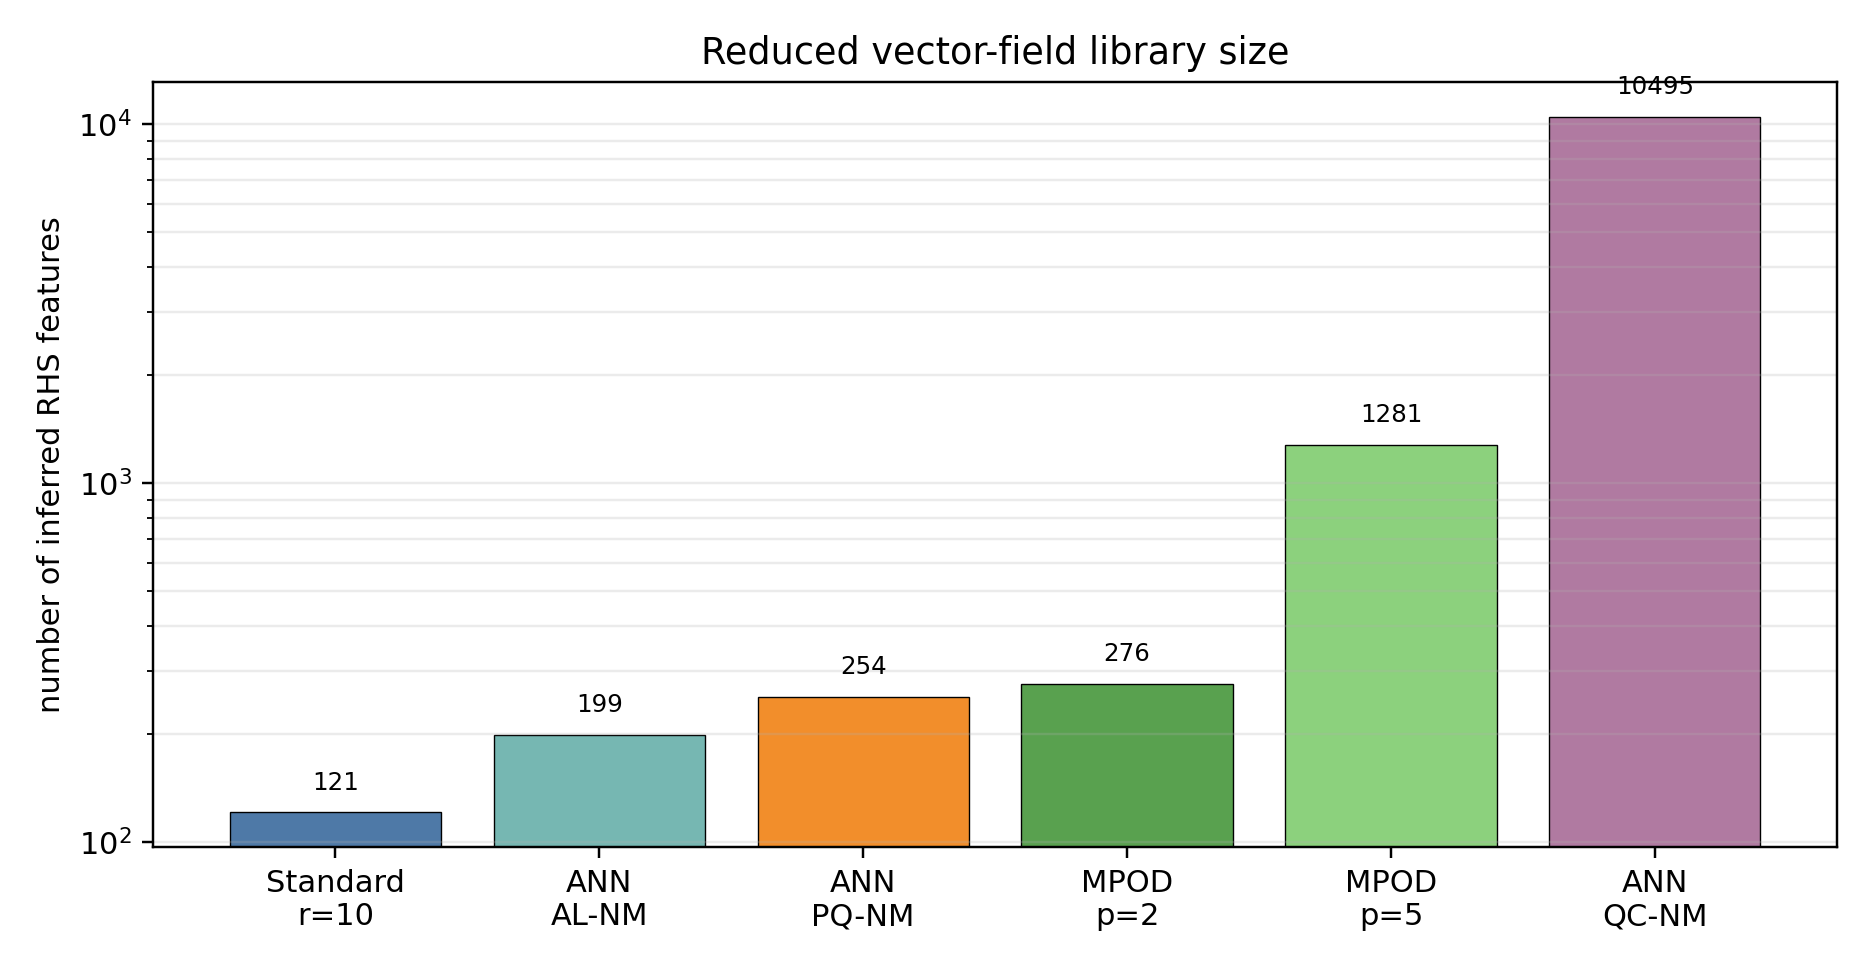
\includegraphics[width=0.78\textwidth]{assets/feature_count_comparison.png}
\caption{Reduced vector-field feature counts for the Burgers models. The
AL- and PQ-NM-MPOD libraries are compact compared with QC-NM-MPOD, but
QC-NM-MPOD is the only algebraically complete quadratic library in the
augmented variables
$[\bq^T,\bz^T]^T$.}
\label{fig:feature_counts}
\end{figure}

\begin{figure}[ht]
\centering
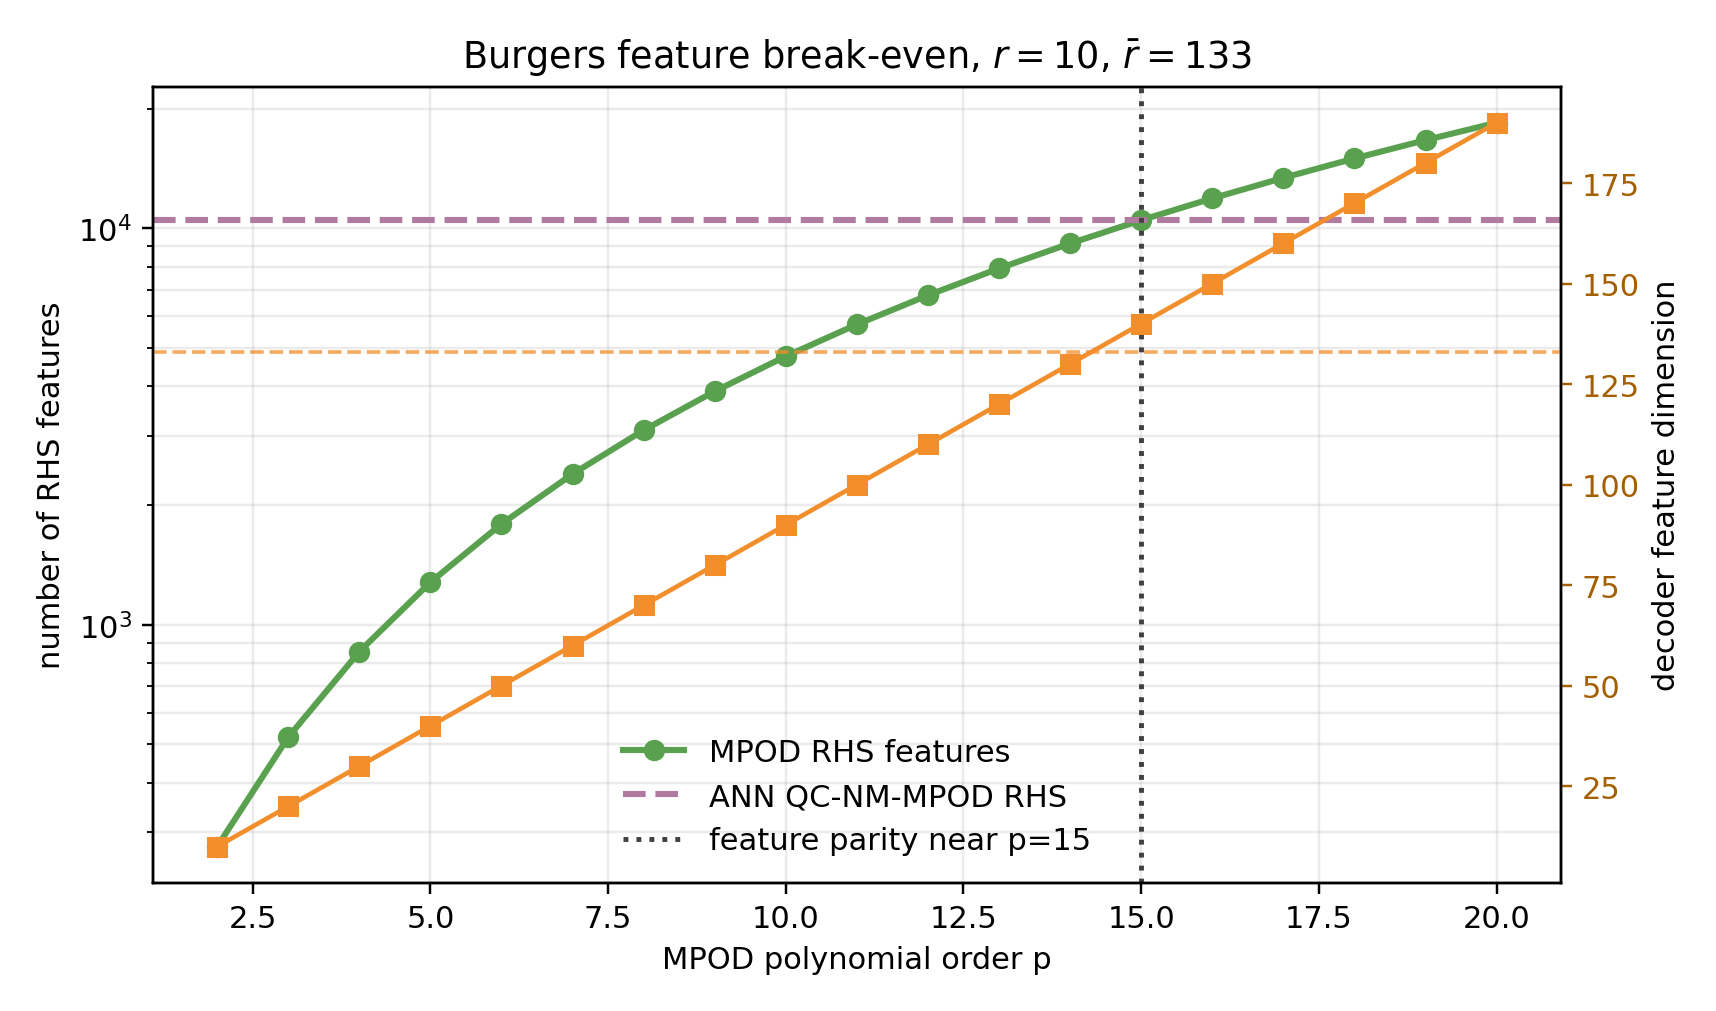
\includegraphics[width=0.78\textwidth]{assets/feature_break_even_analysis.png}
\caption{Feature break-even analysis for Burgers with $\qdim=10$ and
$\rbar=133$. Counting only RHS library features, MPOD reaches the
QC-NM-MPOD feature count near $p=15$. Counting decoder
features only, MPOD also reaches $\rbar=133$ secondary degrees of freedom near
$p=15$ because $\qdim(p-1)=140$. This feature count does not include the ANN
evaluation itself; the ANN adds about $1.43\times10^5$ dense multiply operations
per RHS call before the OpInf feature library is evaluated.}
\label{fig:feature_break_even}
\end{figure}

\section{Numerical evidence}

\subsection{KdV soliton reproduction}

The KdV soliton case was used to verify the standard OpInf, MPOD, and learned
secondary-map machinery on a benchmark close to the nonlinear-manifold OpInf
example studied in \cite{geelen2024learning}. Three GPR-NM-MPOD operator
libraries are retained here: QC-NM-MPOD with
$[1,\bq,\bq_{\mathrm{quad}},\bz,\bq\otimes\bz,\bz_{\mathrm{quad}}]$,
PQ-NM-MPOD with $[1,\bq,\bq_{\mathrm{quad}},\bz(\bq)]$, and AL-NM-MPOD with
$[1,\bq,\bz(\bq)]$. The KdV QC case is therefore the nonparametric GPR analogue
of the Burgers QC ANN experiment, with $\bz=\bz_{\mathrm{GPR}}(\bq)$. For
$\qdim=5$ and $\rbar=9$, the KdV GPR feature counts are $120$ for QC, $30$ for
PQ, and $15$ for AL.

\begin{table}[ht]
\centering
\caption{Representative KdV soliton errors. The training window is
$t\in[0,0.2]$, and the prediction window is
$t\in[0.2,1]$.}
\label{tab:kdv_errors}
\scriptsize
\begin{tabular}{lrrr}
\toprule
Model & Reconstruction/training error & Full-window error & Prediction-window error\\
\midrule
Standard OpInf, $\qdim=5$ & $5.14\times 10^{-1}$ & $5.33\times 10^{-1}$ & $5.37\times 10^{-1}$\\
MPOD-OpInf, $\qdim=5,p=2$ & $4.27\times 10^{-1}$ & $4.44\times 10^{-1}$ & $4.48\times 10^{-1}$\\
GPR QC-NM-MPOD, $\qdim=5,\rbar=9$ & $8.58\times 10^{-2}$ & $8.73\times 10^{-2}$ & $8.77\times 10^{-2}$\\
GPR PQ-NM-MPOD, $\qdim=5,\rbar=9$ & $8.58\times 10^{-2}$ & $8.73\times 10^{-2}$ & $8.77\times 10^{-2}$\\
GPR AL-NM-MPOD, $\qdim=5,\rbar=9$ & $8.58\times 10^{-2}$ & $8.73\times 10^{-2}$ & $8.77\times 10^{-2}$\\
\bottomrule
\end{tabular}
\normalsize
\end{table}

\begin{figure}[ht]
\centering
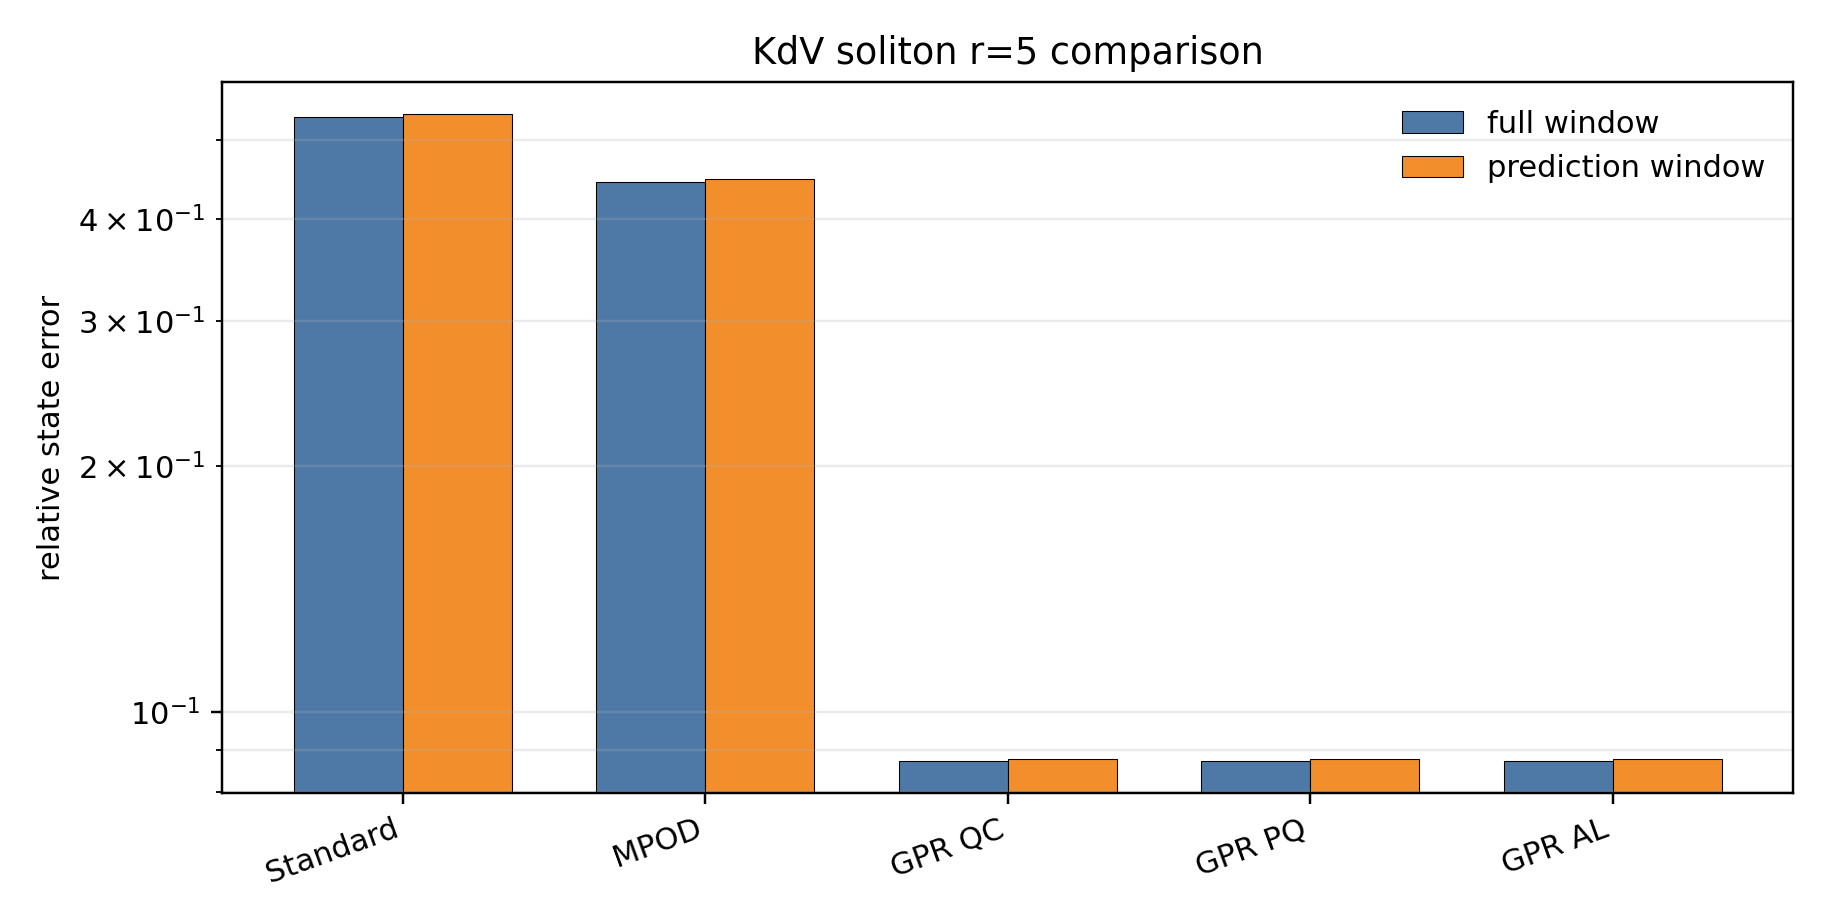
\includegraphics[width=0.78\textwidth]{assets/kdv_error_summary.png}
\caption{KdV soliton $\qdim=5$ summary errors for standard OpInf, MPOD, and
the three retained nonlinear-feature GPR-NM-MPOD variants.}
\label{fig:kdv_errors}
\end{figure}

\begin{figure}[ht]
\centering
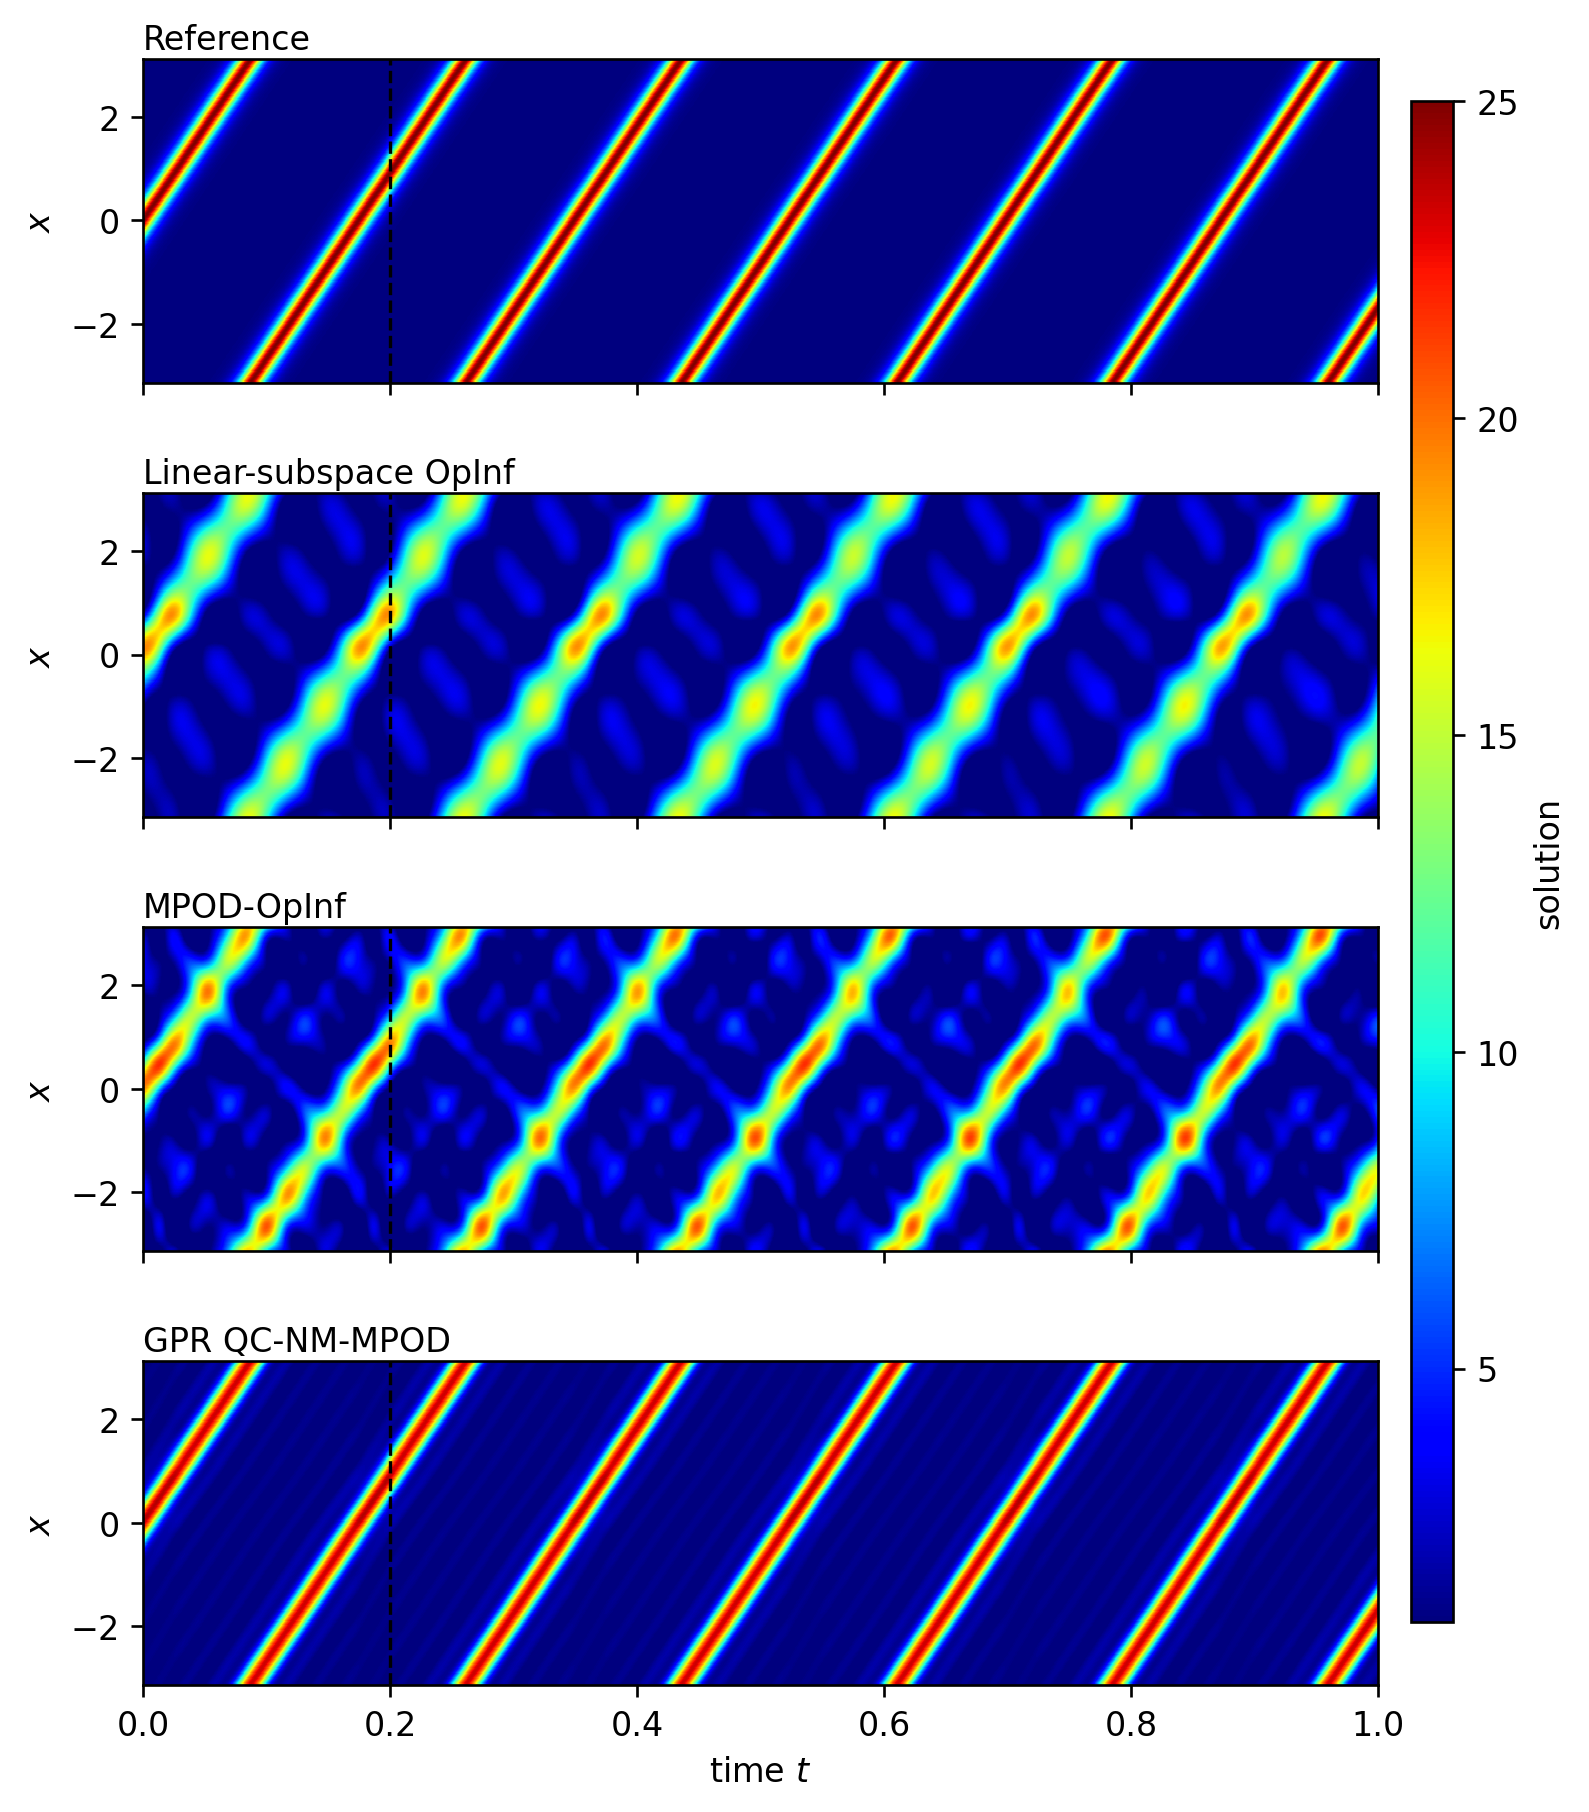
\includegraphics[width=0.84\textwidth]{assets/kdv_reference_linear_mpod_gpr_vertical.png}
\caption{Space-time KdV comparison in a single shared scale: reference,
linear-subspace OpInf, MPOD-OpInf, and the GPR QC-NM-MPOD model.
The dashed vertical line marks the end of the training window at $t=0.2$; the
interval $t\in(0.2,1]$ is prediction.}
\label{fig:kdv_spacetime}
\end{figure}

\subsection{Parametric Burgers test}

The primary evidence for the proposed NM-MPOD idea comes from the parametric
one-dimensional inviscid Burgers problem. The full-order model
uses $N=5000$ finite-volume cells, backward Euler with $\Delta t=0.05$, and
501 snapshots per trajectory. Training snapshots are generated on a $3\times3$
parameter grid:
\[
  \mu_1\in\{4.25,4.875,5.50\},\qquad
  \mu_2\in\{0.015,0.0225,0.030\}.
\]
The three test points are
\[
  (4.56,0.019),\qquad (4.75,0.020),\qquad (5.19,0.026).
\]
These three parameter pairs are not used to fit the POD basis, the MPOD or ANN
secondary-coordinate maps, or the OpInf operators. They are genuine
out-of-sample prediction points in parameter space: each trained ROM is rolled
out at the new parameter value and compared against a separately generated HDM
trajectory.

\begin{figure}[ht]
\centering
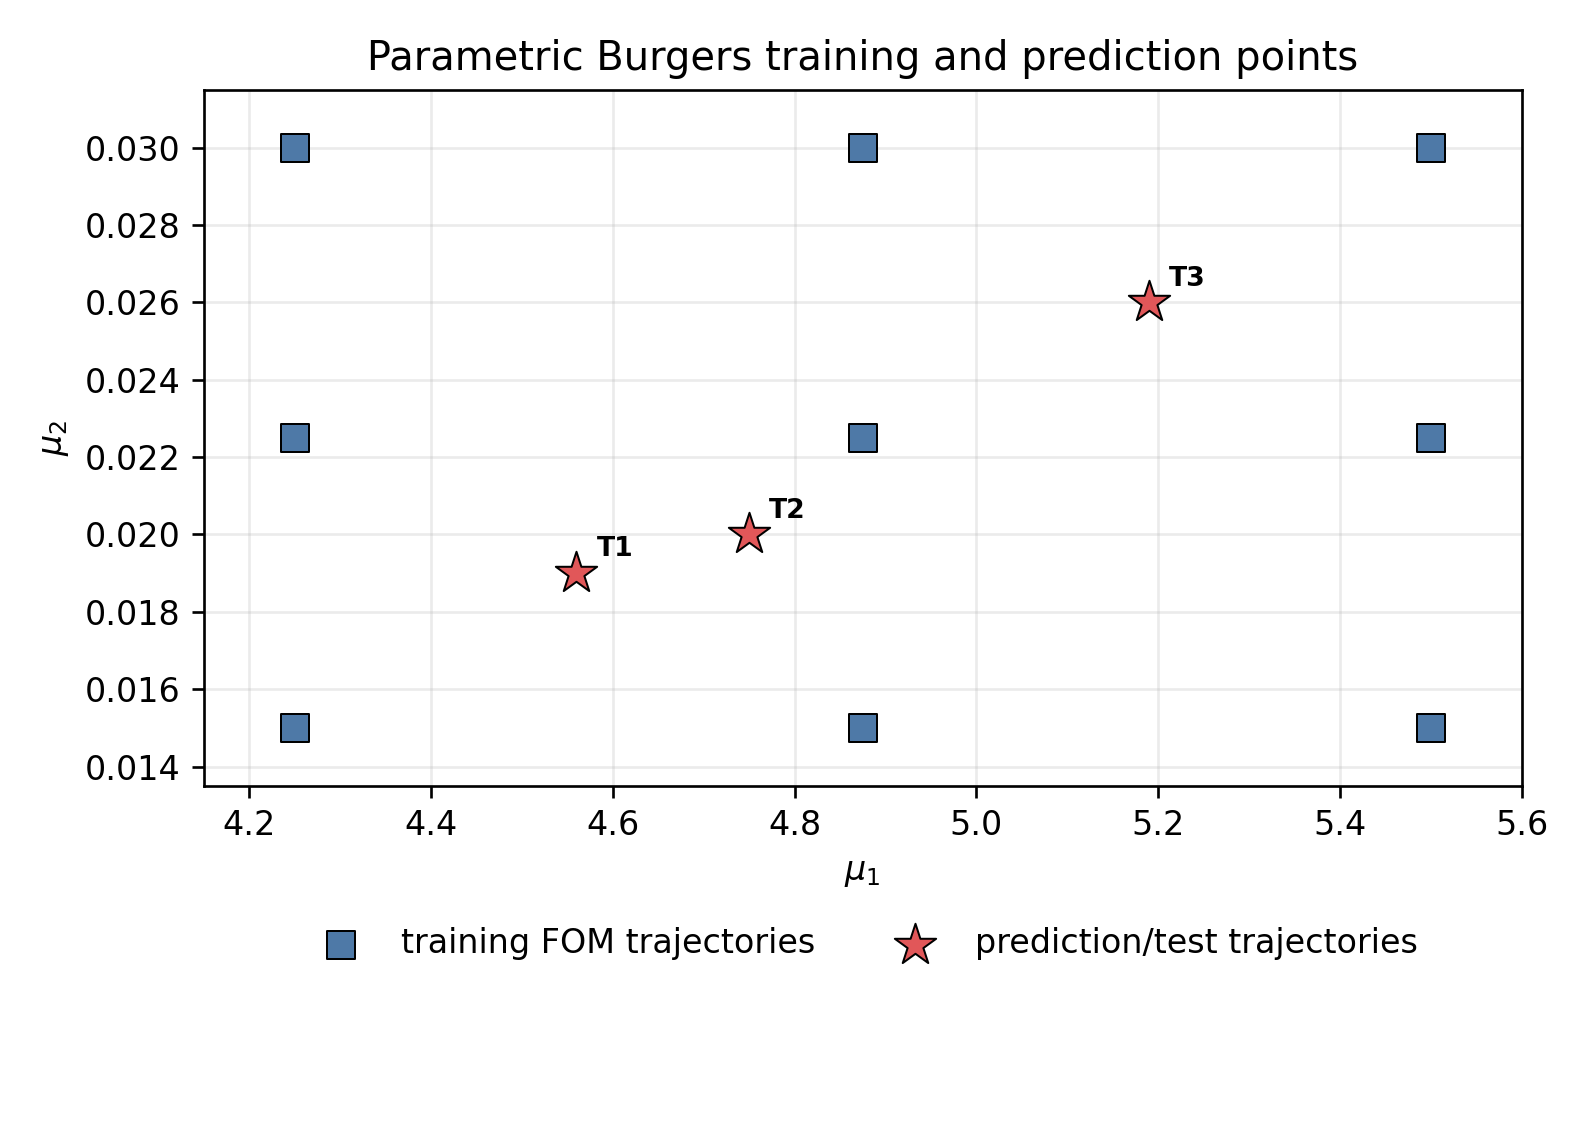
\includegraphics[width=0.70\textwidth]{assets/burgers_parameter_space.png}
\caption{Parametric Burgers training and prediction points. Blue squares are
the nine HDM trajectories used to build the POD basis and fit the reduced
models. Red stars are the three unseen parameter points used only for final
prediction tests.}
\label{fig:burgers_parameter_space}
\end{figure}

\begin{table}[ht]
\centering
\caption{Parametric Burgers relative state errors over all finite rollout
snapshots. All models in this table are continuous-time OpInf models and evolve
$\qdim=10$ coordinates. The ANN-NM-MPOD
decoder uses $\qdim+\rbar=143$ POD modes with $\rbar=133$ secondary coordinates.}
\label{tab:burgers_errors}
\begin{tabular}{lrrr}
\toprule
Model & $(4.56,0.019)$ & $(4.75,0.020)$ & $(5.19,0.026)$\\
\midrule
Standard quadratic OpInf, $\qdim=10$ & $9.11\times10^{-2}$ & $9.11\times10^{-2}$ & $8.74\times10^{-2}$\\
Induced MPOD, $p=2$ & $8.19\times10^{-2}$ & $8.39\times10^{-2}$ & $8.12\times10^{-2}$\\
ANN AL-NM-MPOD & $1.12\times10^{-2}$ & $8.72\times10^{-3}$ & $6.12\times10^{-3}$\\
ANN PQ-NM-MPOD & $1.19\times10^{-2}$ & $1.19\times10^{-2}$ & $1.19\times10^{-2}$\\
ANN QC-NM-MPOD & $5.97\times10^{-3}$ & $5.76\times10^{-3}$ & $6.56\times10^{-3}$\\
\bottomrule
\end{tabular}
\end{table}

\begin{table}[ht]
\centering
\caption{Burgers MPOD polynomial-order sensitivity with
$\qdim=10$ and $\rbar=133$. Increasing the polynomial order improves the MPOD
rollout errors only modestly while substantially increasing the inferred
feature dimension.}
\label{tab:burgers_mpod_order}
\begin{tabular}{lrrrr}
\toprule
MPOD order & RHS features & $(4.56,0.019)$ & $(4.75,0.020)$ & $(5.19,0.026)$\\
\midrule
$p=2$ & 276 & $8.19\times10^{-2}$ & $8.39\times10^{-2}$ & $8.12\times10^{-2}$\\
$p=4$ & 856 & $7.75\times10^{-2}$ & $8.30\times10^{-2}$ & $8.11\times10^{-2}$\\
$p=5$ & 1281 & $7.61\times10^{-2}$ & $8.29\times10^{-2}$ & $7.97\times10^{-2}$\\
\bottomrule
\end{tabular}
\end{table}

\begin{figure}[ht]
\centering
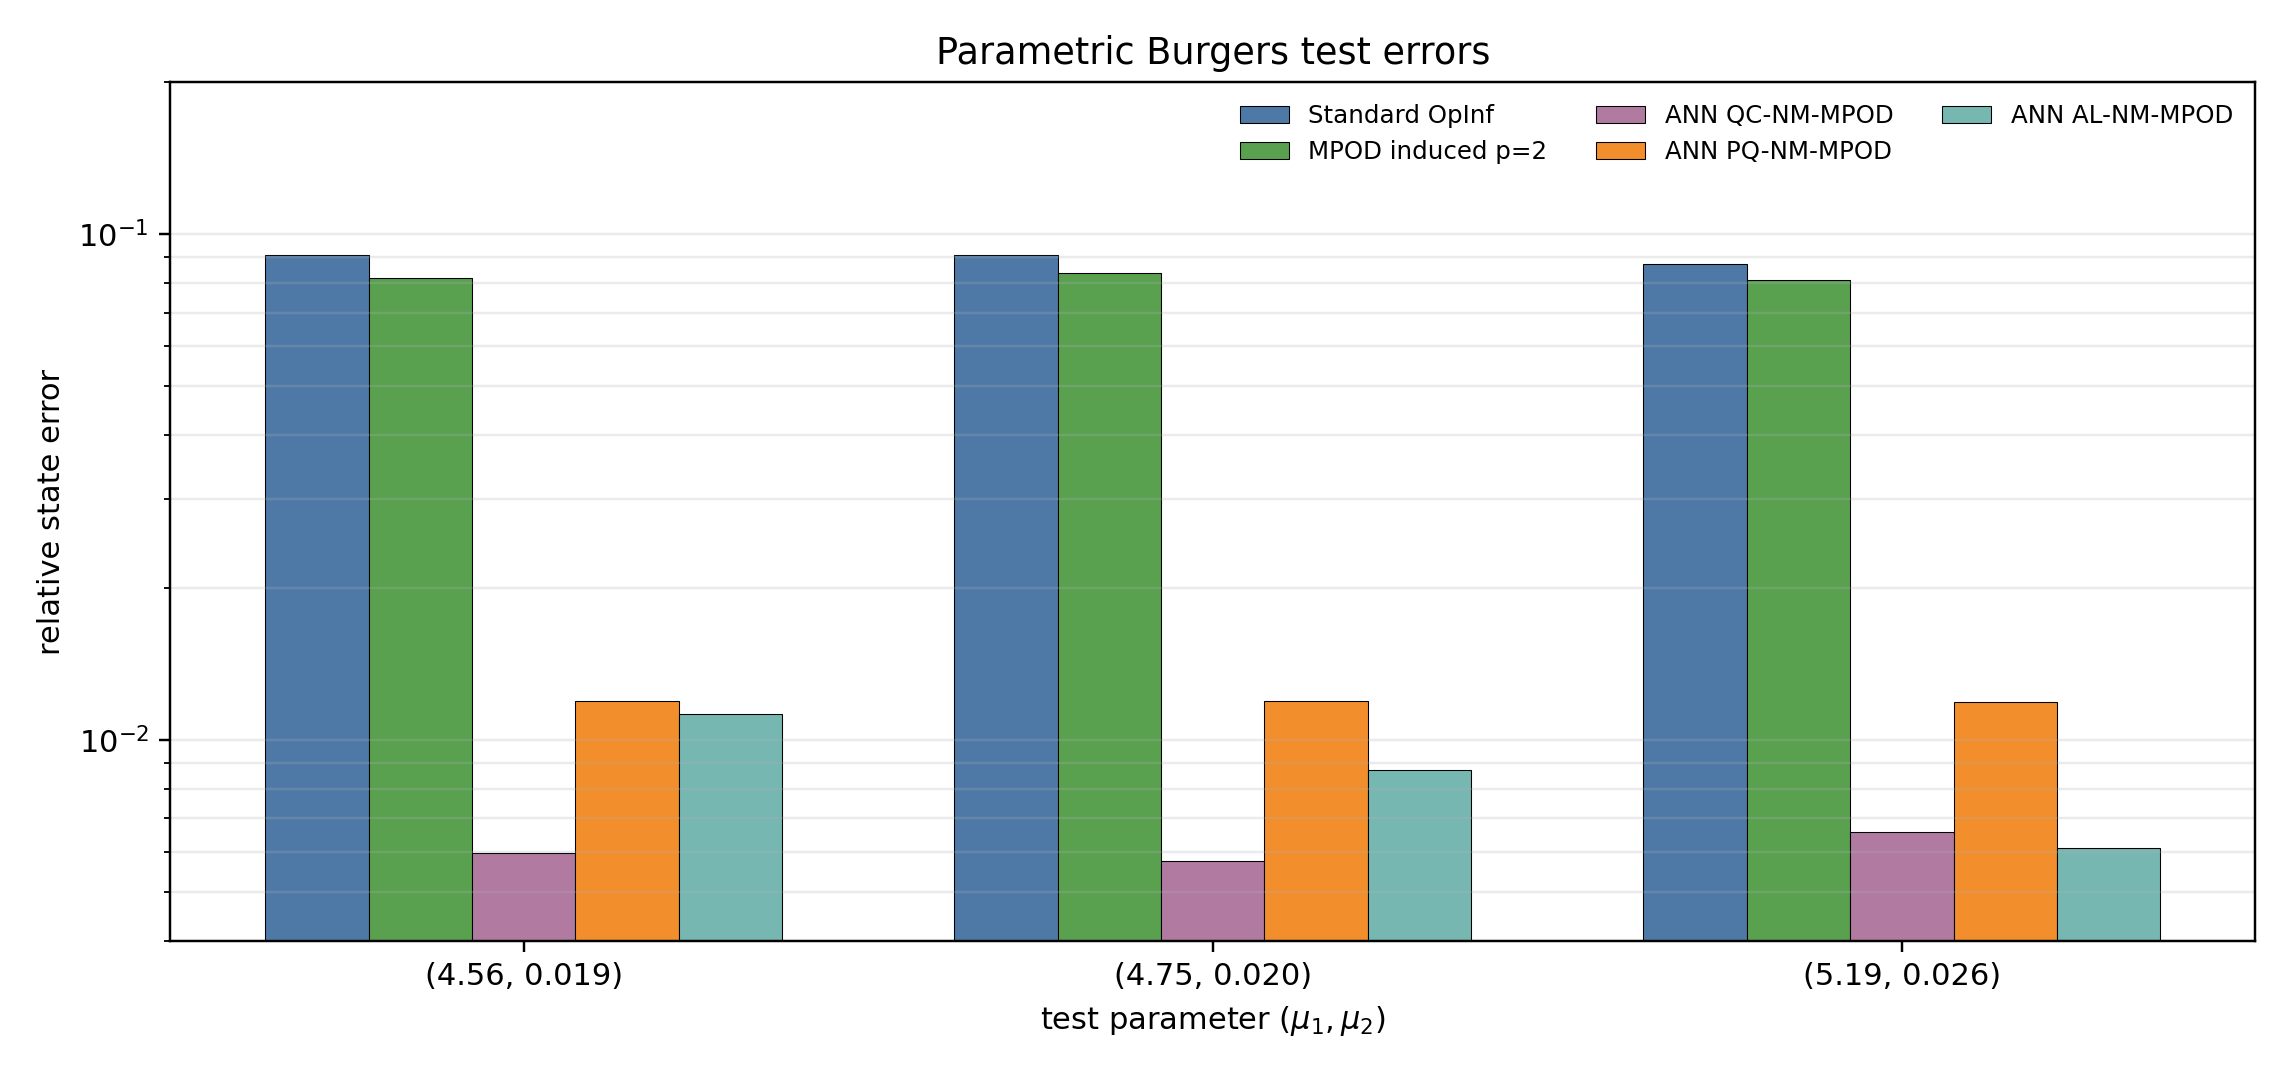
\includegraphics[width=\textwidth]{assets/burgers_error_comparison.png}
\caption{Parametric Burgers test errors. The ANN QC-NM-MPOD model gives the
lowest average continuous-time error in the retained suite; the AL variant is
cheaper and competitive, and is
best at the third test point.}
\label{fig:burgers_errors}
\end{figure}

\begin{figure}[ht]
\centering
\begin{subfigure}{0.32\textwidth}
  \centering
  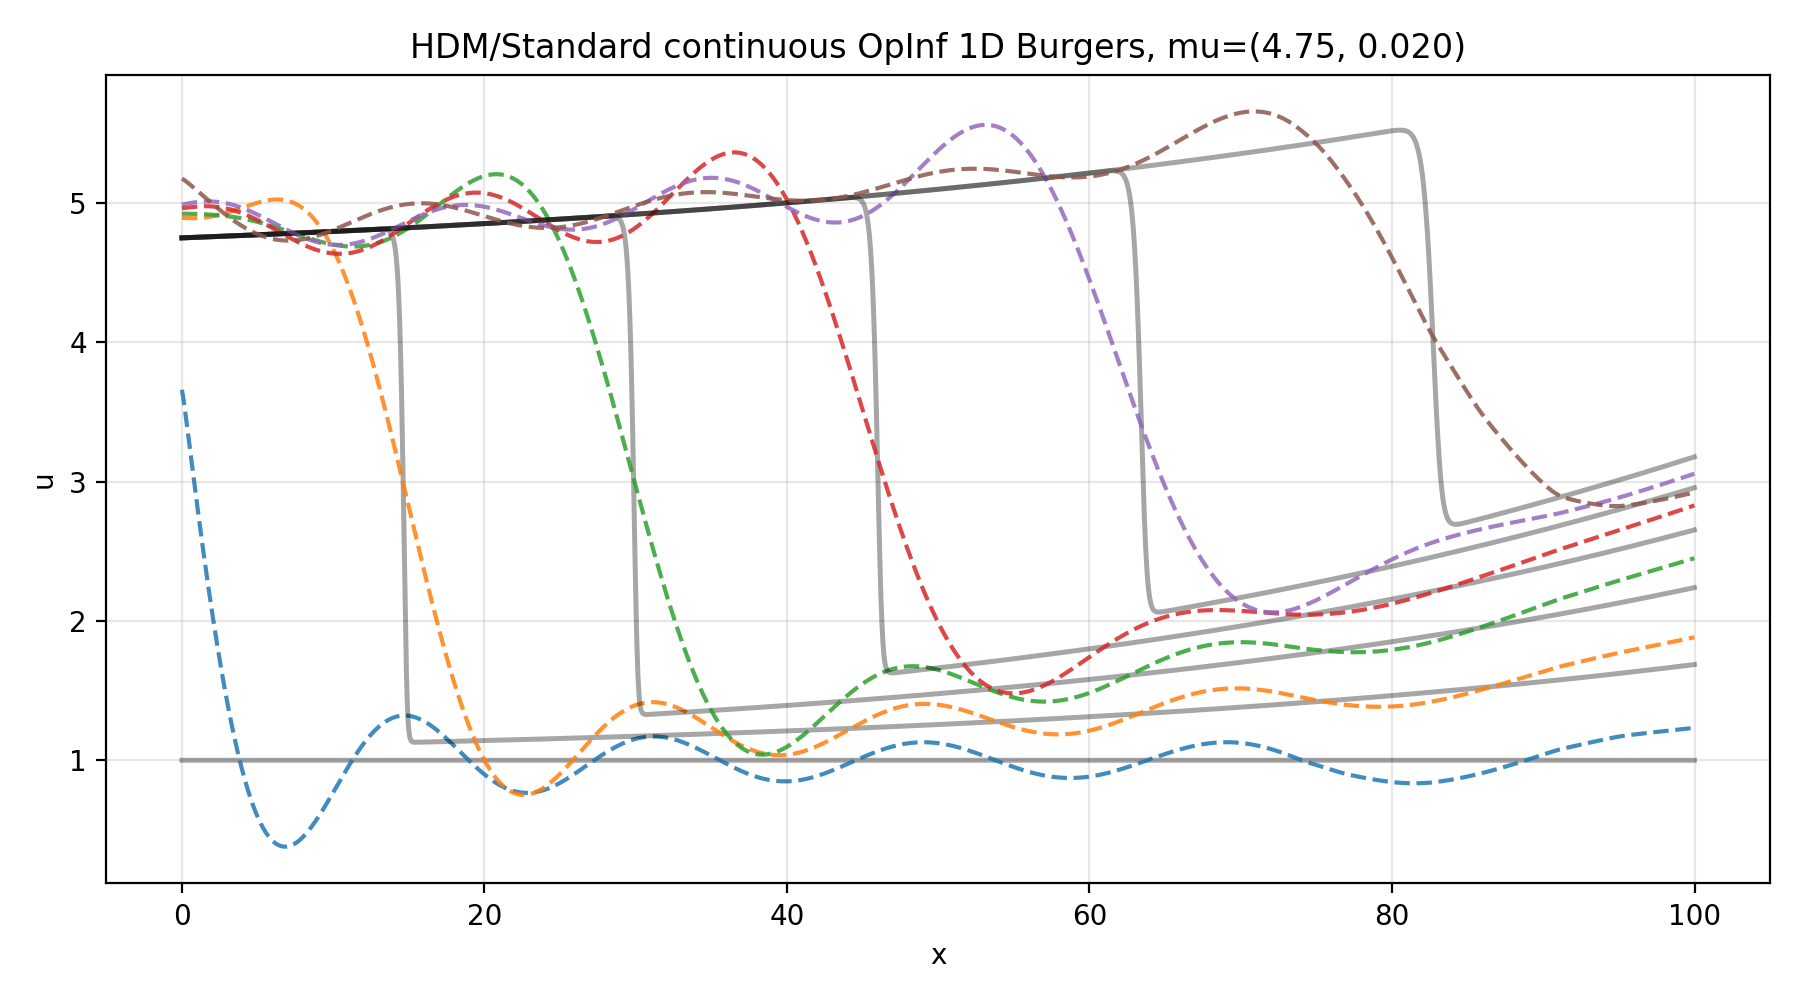
\includegraphics[width=\textwidth]{assets/burgers_standard_mu475.png}
  \caption{Standard OpInf.}
\end{subfigure}
\begin{subfigure}{0.32\textwidth}
  \centering
  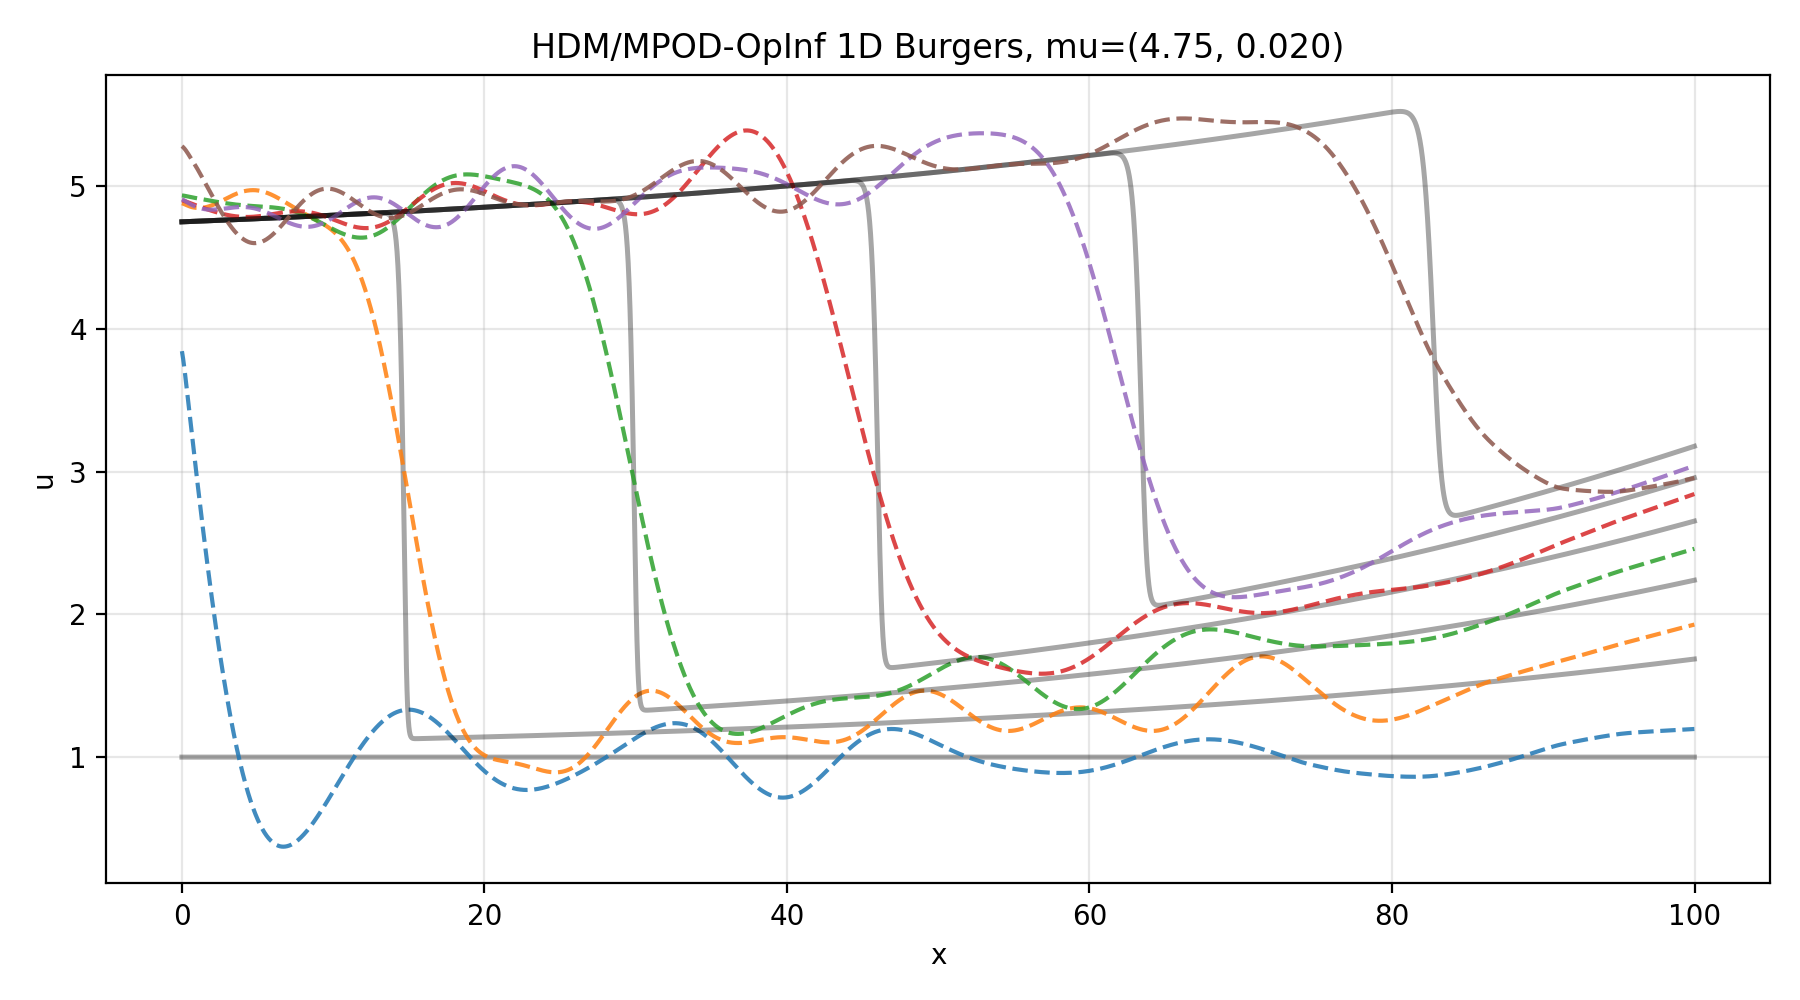
\includegraphics[width=\textwidth]{assets/burgers_mpod_p2_mu475.png}
  \caption{Induced MPOD, $p=2$.}
\end{subfigure}
\begin{subfigure}{0.32\textwidth}
  \centering
  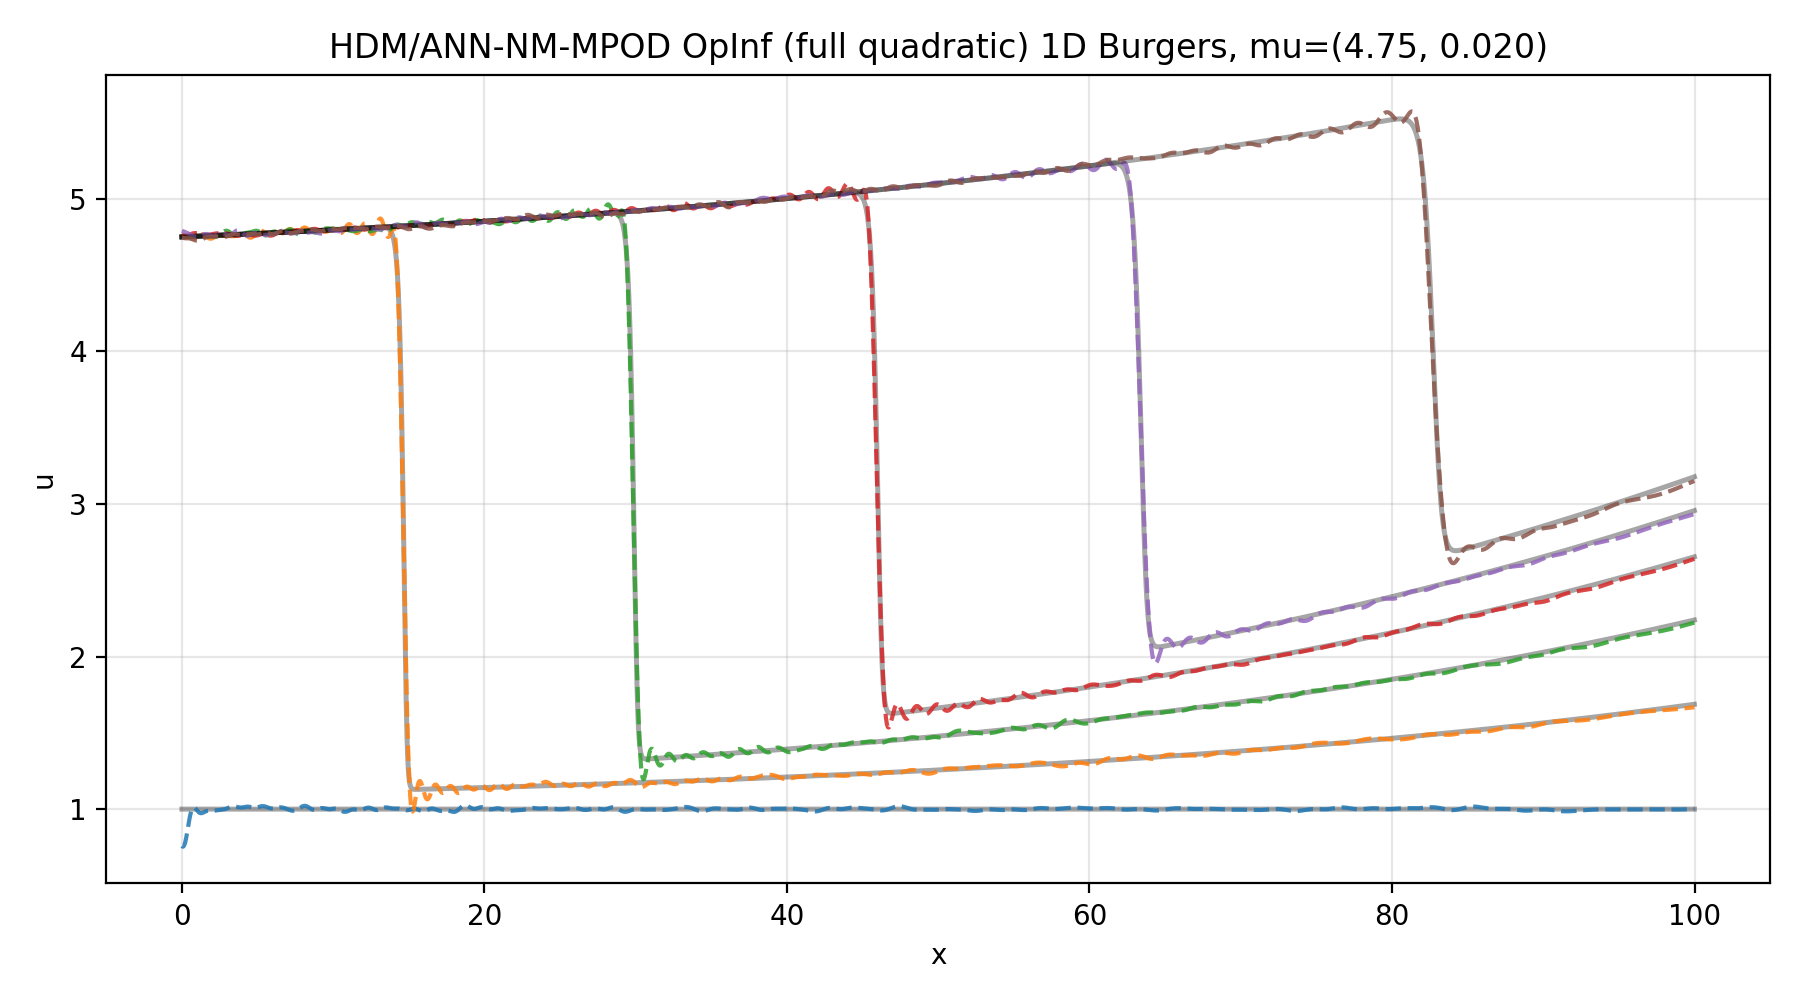
\includegraphics[width=\textwidth]{assets/burgers_fullquad_mu475.png}
  \caption{ANN QC-NM-MPOD.}
\end{subfigure}
\caption{Representative Burgers rollout overlays at $\mu=(4.75,0.020)$. The
induced MPOD model improves strongly on the linear-subspace standard model, and
the ANN QC-NM-MPOD decoder/operator pair gives the smallest continuous-time
error in this comparison.}
\label{fig:burgers_overlay}
\end{figure}

\begin{figure}[ht]
\centering
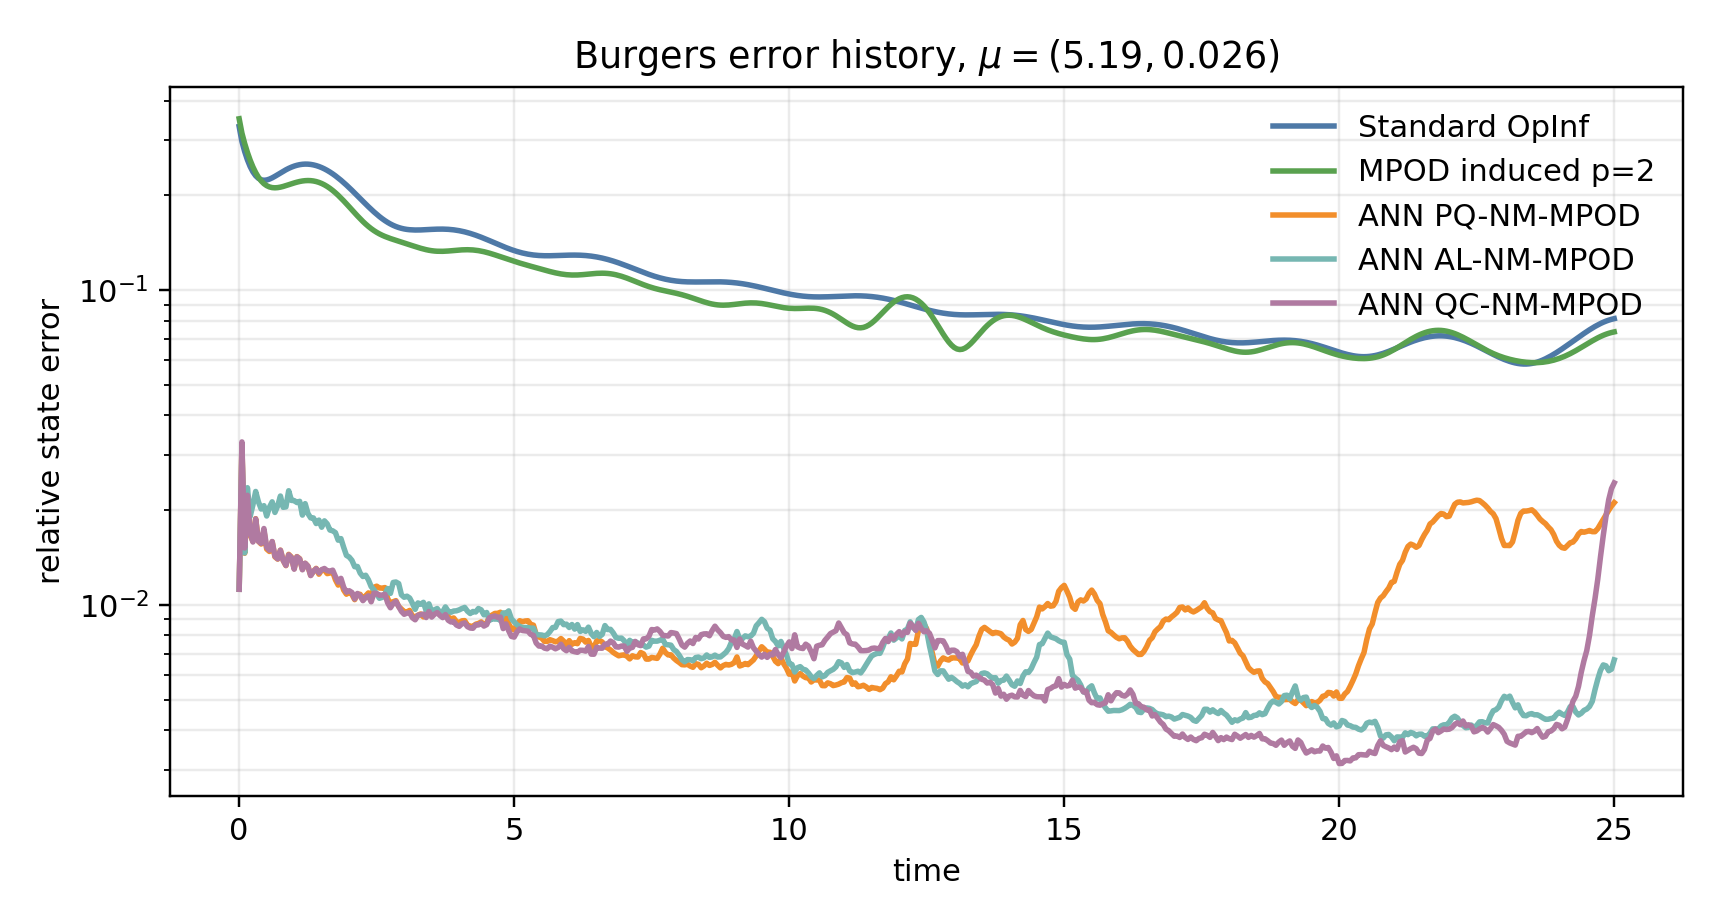
\includegraphics[width=0.82\textwidth]{assets/burgers_error_history_comparison_mu519.png}
\caption{Error histories at $\mu=(5.19,0.026)$ for the retained continuous-time
Burgers comparison.}
\label{fig:burgers_error_history}
\end{figure}

\section{Interpretation}

The retained Burgers results support three conclusions.

\paragraph{1. The nonlinear map is the decisive improvement in this retained
Burgers configuration.}
The standard $\qdim=10$ linear-subspace OpInf model has errors of order
$8.7\times10^{-2}$ to $9.1\times10^{-2}$. Induced MPOD with $p=2$ reduces these
errors only modestly, to roughly $8.1\times10^{-2}$ to $8.4\times10^{-2}$. The
AL-, PQ-, and QC-NM-MPOD models all reduce the errors by roughly one order of
magnitude relative to MPOD. The QC model gives errors of roughly
$5.8\times10^{-3}$ to $6.6\times10^{-3}$, while the AL model gives
$6.1\times10^{-3}$ to $1.1\times10^{-2}$.
The MPOD order sweep in Table~\ref{tab:burgers_mpod_order} shows that increasing
$p$ from 2 to 5 gives only a small additional improvement. Thus, for this
Burgers configuration, the main gain appears to come from the learned secondary
map. The mixed/secondary quadratic operator blocks improve the mean test error,
but the AL result shows that the decoder itself is already carrying a large
part of the gain.

\paragraph{2. Burgers MPOD is now the same kind of MPOD as the KdV MPOD.}
The Burgers MPOD ODE no longer appends only the decoder powers $g_p(\bq)$. It
uses the induced library $\hat{\boldsymbol g}(\bq)$ generated by substituting
$\bXi\boldsymbol g_p(\bq)$ into a quadratic full-order vector field. Thus the KdV and
Burgers MPOD tests now use the same theoretical construction, with the Burgers
library additionally carrying the parameter blocks
$\boldeta(\bmu)$ and $\boldeta(\bmu)\otimes\bq$.

\paragraph{3. QC-NM-MPOD is the algebraically complete quadratic model, while
AL-NM-MPOD is the cheapest competitive variant.}
The ANN QC-NM-MPOD model uses the algebraically complete quadratic library
\[
  [1,\boldeta,\bq,\boldeta\otimes\bq,\bq_{\mathrm{quad}},
  \bz,\bq\otimes\bz,\bz_{\mathrm{quad}}],
  \qquad \bz=\Nmap(\bq,\bmu),
\]
and gives the lowest average error over the three Burgers test points. The
AL variant removes $\bq_{\mathrm{quad}}$, $\bq\otimes\bz$, and
$\bz_{\mathrm{quad}}$ from the dynamics library, reducing the RHS feature count
from $10495$ to $199$, while remaining competitive and even giving the lowest
error at the third test point. This is useful evidence that two effects should
be separated in future work: the accuracy of the learned nonlinear decoder and
the algebraic completeness of the inferred vector-field library.

\section{Scope and proposed next steps}

The present results are promising and internally consistent, but they should be
read as a preliminary numerical study. A mature journal submission should
resolve the following research questions.

\begin{enumerate}
  \item \textbf{Tangent-aware vs. modal projection.} Should NM-MPOD use the
  same $\bV^T$ modal projection implicit in the retained OpInf structure, or should
  it use a tangent-space projection involving $\bJ_\Gamma(\bq)$? The latter is more
  geometrically faithful but less nonintrusive and more expensive for ANN maps.

  \item \textbf{Block-regularized QC libraries.} The QC library
  should be learned with separate penalties for $\bq$, $\bz$, $\bq\otimes\bq$,
  $\bq\otimes\bz$, and $\bz\otimes\bz$. A single scalar ridge parameter is too blunt for
  terms with very different scales and dimensions.

  \item \textbf{Compressed mixed and secondary quadratic terms.} Instead of
  using all 1330 $\bq\otimes\bz$ and 8911 $\bz\otimes\bz$ terms, one can SVD-compress
  these feature blocks, use randomized sketches, or infer a low-rank operator
  factorization.

  \item \textbf{Parameter-complete libraries.} The retained Burgers
  QC model is state-quadratically complete but not fully
  parameter-complete. Additional tests should include $\boldeta\otimes\bz$ and
  possibly $\boldeta\otimes(\bq\otimes\bz)$ terms if the inferred operator is intended
  to represent broad parametric dependence.

  \item \textbf{Decoder uncertainty and validation.} Gaussian-process and RBF versions of
  $\Nmap$ are useful when data are sparse. GPR uncertainty could be used to
  detect rollout regions where the ROM leaves the training manifold.

  \item \textbf{Broader benchmarks.} The present evidence covers KdV and
  parametric inviscid Burgers. A convincing paper would need additional
  transport-dominated and nonlinear PDE tests, plus systematic sweeps in
  $(r,\bar r)$ and training-set size.
\end{enumerate}

\section{Experimental protocol}

All numerical results follow the same nonintrusive workflow. First, HDM
snapshots are centered by the reference state and compressed by POD. Second, the
primary and secondary coordinates are separated according to the prescribed
values of $\qdim$ and $\rbar$. Third, the secondary-coordinate decoder is fit
from training snapshots only. Fourth, the reduced vector field is inferred by
regularized continuous-time OpInf using the feature library associated with the
chosen model class. Finally, the reduced ODE is initialized from the projected
HDM initial condition and integrated over the full prediction horizon without
access to the reference trajectory.

For Burgers, the regularization and time-integration hyperparameters are selected
using rollout errors on training trajectories; the three parameter points in
Table~\ref{tab:burgers_errors} are held out until the final comparison. For KdV,
the training interval is $t\in[0,0.2]$ and the interval $t\in(0.2,1]$ is used to
assess extrapolation in time. These protocols separate model construction from
the reported prediction tests and avoid using the plotted test trajectories for
operator fitting.

\section{Conclusion}

The NM-MPOD idea is a natural extension of nonlinear-manifold OpInf: retain the
modal primary/secondary split of MPOD, but replace the fixed polynomial
secondary-coordinate map by a learned nonlinear map. This keeps the online ODE
dimension small while allowing the decoder to represent transport-dominated
state geometry more effectively than a low-dimensional linear subspace.

For quadratic PDEs under the modal-projection formulation used here, the
quadratic completion is clear:
$\bq\otimes \bq$, $\bq\otimes \Nmap$, and
$\Nmap\otimes\Nmap$ must be included in the QC-NM-MPOD operator library. The
numerical evidence here shows that QC-NM-MPOD combined with an ANN
secondary-coordinate map gives the best average continuous-time Burgers error
among the retained models, while AL-NM-MPOD is a much cheaper competitive
alternative. The next research direction is to learn nonlinear-map manifold
decoders and infer compressed, block-regularized, physics-structured reduced
operators on top of them.

\begin{thebibliography}{9}

\bibitem{peherstorfer2016opinf}
B. Peherstorfer and K. Willcox.
\newblock Data-driven operator inference for nonintrusive projection-based
model reduction.
\newblock \emph{Computer Methods in Applied Mechanics and Engineering},
306:196--215, 2016.

\bibitem{geelen2022quad}
R. Geelen, S. Wright, and K. Willcox.
\newblock Operator inference for non-intrusive model reduction with quadratic
manifolds.
\newblock arXiv:2205.02304, 2022.
\newblock \url{https://arxiv.org/abs/2205.02304}.

\bibitem{geelen2024learning}
R. Geelen, L. Balzano, S. Wright, and K. Willcox.
\newblock Learning physics-based reduced-order models from data using nonlinear
manifolds.
\newblock arXiv:2308.02802v2, 2024.
\newblock \url{https://arxiv.org/abs/2308.02802}.

\end{thebibliography}

\end{document}
